% ------------------------------------------------------------------------------------------------------------------
% Basic configuration and packages
% ------------------------------------------------------------------------------------------------------------------
% Package for discovering wrong and outdated usage of LaTeX.
% More information to be found in l2tabu English version.
\RequirePackage[l2tabu, orthodox]{nag}
% Class of LaTeX document: {size of paper, size of font}[document class]
\documentclass[a4paper,11pt]{article}



% ------------------------------------------------------
% Packages not tied to particular normal language
% ------------------------------------------------------
% This package should improved spaces in the text
\usepackage{microtype}
% Add few important symbols, like text Celcius degree
\usepackage{textcomp}



% ------------------------------------------------------
% Polonization of LaTeX document
% ------------------------------------------------------
% Basic polonization of the text
\usepackage[MeX]{polski}
% Switching on UTF-8 encoding
\usepackage[utf8]{inputenc}
% Adding font Latin Modern
\usepackage{lmodern}
% Package is need for fonts Latin Modern
\usepackage[T1]{fontenc}



% ------------------------------------------------------
% Setting margins
% ------------------------------------------------------
\usepackage[a4paper, total={14cm, 25cm}]{geometry}



% ------------------------------------------------------
% Setting vertical spaces in the text
% ------------------------------------------------------
% Setting space between lines
\renewcommand{\baselinestretch}{1.1}

% Setting space between lines in tables
\renewcommand{\arraystretch}{1.4}



% ------------------------------------------------------
% Packages for scientific papers
% ------------------------------------------------------
% Switching off \lll symbol, that I guess is representing letter "Ł"
% It collide with `amsmath' package's command with the same name
\let\lll\undefined
% Basic package from American Mathematical Society (AMS)
\usepackage[intlimits]{amsmath}
% Equations are numbered separately in every section
\numberwithin{equation}{section}

% Other very useful packages from AMS
\usepackage{amsfonts}
\usepackage{amssymb}
\usepackage{amscd}
\usepackage{amsthm}

% Package with better looking calligraphy fonts
\usepackage{calrsfs}

% Package with better looking greek letters
% Example of use: pi -> \uppi
\usepackage{upgreek}
% Improving look of lambda letter
\let\oldlambda\lambda
\renewcommand{\lambda}{\uplambda}




% ------------------------------------------------------
% BibLaTeX
% ------------------------------------------------------
% Package biblatex, with biber as its backend, allow us to handle
% bibliography entries that use Unicode symbols outside ASCII
% \usepackage[
% language=polish,
% backend=biber,
% style=alphabetic,
% url=false,
% eprint=true,
% ]{biblatex}

% \addbibresource{Logika-i-teoria-mnogości-Bibliography.bib}





% ------------------------------------------------------
% Defining new environments (?)
% ------------------------------------------------------
% Defining enviroment "Wniosek"
% \newtheorem{corollary}{Wniosek}
% \newtheorem{definition}{Definicja}
% \newtheorem{theorem}{Twierdzenie}





% ------------------------------------------------------
% xcolor, the main LaTeX color package
% ------------------------------------------------------

\usepackage{xcolor}

% Defining colors in RGB system
\definecolor{colorR0G0B0}{RGB}{0, 0, 0}
\definecolor{colorR1G0B0}{RGB}{1, 0, 0}
\definecolor{colorR2G0B0}{RGB}{2, 0, 0}
\definecolor{colorR3G0B0}{RGB}{3, 0, 0}
\definecolor{colorR4G0B0}{RGB}{4, 0, 0}
\definecolor{colorR5G0B0}{RGB}{5, 0, 0}
\definecolor{colorR6G0B0}{RGB}{6, 0, 0}
\definecolor{colorR7G0B0}{RGB}{7, 0, 0}
\definecolor{colorR8G0B0}{RGB}{8, 0, 0}
\definecolor{colorR9G0B0}{RGB}{9, 0, 0}
\definecolor{colorR10G0B0}{RGB}{10, 0, 0}
\definecolor{colorR11G0B0}{RGB}{11, 0, 0}
\definecolor{colorR12G0B0}{RGB}{12, 0, 0}
\definecolor{colorR13G0B0}{RGB}{13, 0, 0}
\definecolor{colorR14G0B0}{RGB}{14, 0, 0}
\definecolor{colorR15G0B0}{RGB}{15, 0, 0}
\definecolor{colorR16G0B0}{RGB}{16, 0, 0}
\definecolor{colorR17G0B0}{RGB}{17, 0, 0}
\definecolor{colorR18G0B0}{RGB}{18, 0, 0}
\definecolor{colorR19G0B0}{RGB}{19, 0, 0}
\definecolor{colorR20G0B0}{RGB}{20, 0, 0}
\definecolor{colorR21G0B0}{RGB}{21, 0, 0}
\definecolor{colorR22G0B0}{RGB}{22, 0, 0}
\definecolor{colorR23G0B0}{RGB}{23, 0, 0}
\definecolor{colorR24G0B0}{RGB}{24, 0, 0}
\definecolor{colorR25G0B0}{RGB}{25, 0, 0}
\definecolor{colorR26G0B0}{RGB}{26, 0, 0}
\definecolor{colorR27G0B0}{RGB}{27, 0, 0}
\definecolor{colorR28G0B0}{RGB}{28, 0, 0}
\definecolor{colorR29G0B0}{RGB}{29, 0, 0}
\definecolor{colorR30G0B0}{RGB}{30, 0, 0}
\definecolor{colorR31G0B0}{RGB}{31, 0, 0}
\definecolor{colorR32G0B0}{RGB}{32, 0, 0}
\definecolor{colorR33G0B0}{RGB}{33, 0, 0}
\definecolor{colorR34G0B0}{RGB}{34, 0, 0}
\definecolor{colorR35G0B0}{RGB}{35, 0, 0}
\definecolor{colorR36G0B0}{RGB}{36, 0, 0}
\definecolor{colorR37G0B0}{RGB}{37, 0, 0}
\definecolor{colorR38G0B0}{RGB}{38, 0, 0}
\definecolor{colorR39G0B0}{RGB}{39, 0, 0}
\definecolor{colorR40G0B0}{RGB}{40, 0, 0}
\definecolor{colorR41G0B0}{RGB}{41, 0, 0}
\definecolor{colorR42G0B0}{RGB}{42, 0, 0}
\definecolor{colorR43G0B0}{RGB}{43, 0, 0}
\definecolor{colorR44G0B0}{RGB}{44, 0, 0}
\definecolor{colorR45G0B0}{RGB}{45, 0, 0}
\definecolor{colorR46G0B0}{RGB}{46, 0, 0}
\definecolor{colorR47G0B0}{RGB}{47, 0, 0}
\definecolor{colorR48G0B0}{RGB}{48, 0, 0}
\definecolor{colorR49G0B0}{RGB}{49, 0, 0}
\definecolor{colorR50G0B0}{RGB}{50, 0, 0}
\definecolor{colorR51G0B0}{RGB}{51, 0, 0}
\definecolor{colorR52G0B0}{RGB}{52, 0, 0}
\definecolor{colorR53G0B0}{RGB}{53, 0, 0}
\definecolor{colorR54G0B0}{RGB}{54, 0, 0}
\definecolor{colorR55G0B0}{RGB}{55, 0, 0}
\definecolor{colorR56G0B0}{RGB}{56, 0, 0}
\definecolor{colorR57G0B0}{RGB}{57, 0, 0}
\definecolor{colorR58G0B0}{RGB}{58, 0, 0}
\definecolor{colorR59G0B0}{RGB}{59, 0, 0}
\definecolor{colorR60G0B0}{RGB}{60, 0, 0}
\definecolor{colorR61G0B0}{RGB}{61, 0, 0}
\definecolor{colorR62G0B0}{RGB}{62, 0, 0}
\definecolor{colorR63G0B0}{RGB}{63, 0, 0}
\definecolor{colorR64G0B0}{RGB}{64, 0, 0}
\definecolor{colorR65G0B0}{RGB}{65, 0, 0}
\definecolor{colorR66G0B0}{RGB}{66, 0, 0}
\definecolor{colorR67G0B0}{RGB}{67, 0, 0}
\definecolor{colorR68G0B0}{RGB}{68, 0, 0}
\definecolor{colorR69G0B0}{RGB}{69, 0, 0}
\definecolor{colorR70G0B0}{RGB}{70, 0, 0}
\definecolor{colorR71G0B0}{RGB}{71, 0, 0}
\definecolor{colorR72G0B0}{RGB}{72, 0, 0}
\definecolor{colorR73G0B0}{RGB}{73, 0, 0}
\definecolor{colorR74G0B0}{RGB}{74, 0, 0}
\definecolor{colorR75G0B0}{RGB}{75, 0, 0}
\definecolor{colorR76G0B0}{RGB}{76, 0, 0}
\definecolor{colorR77G0B0}{RGB}{77, 0, 0}
\definecolor{colorR78G0B0}{RGB}{78, 0, 0}
\definecolor{colorR79G0B0}{RGB}{79, 0, 0}
\definecolor{colorR80G0B0}{RGB}{80, 0, 0}
\definecolor{colorR81G0B0}{RGB}{81, 0, 0}
\definecolor{colorR82G0B0}{RGB}{82, 0, 0}
\definecolor{colorR83G0B0}{RGB}{83, 0, 0}
\definecolor{colorR84G0B0}{RGB}{84, 0, 0}
\definecolor{colorR85G0B0}{RGB}{85, 0, 0}
\definecolor{colorR86G0B0}{RGB}{86, 0, 0}
\definecolor{colorR87G0B0}{RGB}{87, 0, 0}
\definecolor{colorR88G0B0}{RGB}{88, 0, 0}
\definecolor{colorR89G0B0}{RGB}{89, 0, 0}
\definecolor{colorR90G0B0}{RGB}{90, 0, 0}
\definecolor{colorR91G0B0}{RGB}{91, 0, 0}
\definecolor{colorR92G0B0}{RGB}{92, 0, 0}
\definecolor{colorR93G0B0}{RGB}{93, 0, 0}
\definecolor{colorR94G0B0}{RGB}{94, 0, 0}
\definecolor{colorR95G0B0}{RGB}{95, 0, 0}
\definecolor{colorR96G0B0}{RGB}{96, 0, 0}
\definecolor{colorR97G0B0}{RGB}{97, 0, 0}
\definecolor{colorR98G0B0}{RGB}{98, 0, 0}
\definecolor{colorR99G0B0}{RGB}{99, 0, 0}
\definecolor{colorR100G0B0}{RGB}{100, 0, 0}
\definecolor{colorR101G0B0}{RGB}{101, 0, 0}
\definecolor{colorR102G0B0}{RGB}{102, 0, 0}
\definecolor{colorR103G0B0}{RGB}{103, 0, 0}
\definecolor{colorR104G0B0}{RGB}{104, 0, 0}
\definecolor{colorR105G0B0}{RGB}{105, 0, 0}
\definecolor{colorR106G0B0}{RGB}{106, 0, 0}
\definecolor{colorR107G0B0}{RGB}{107, 0, 0}
\definecolor{colorR108G0B0}{RGB}{108, 0, 0}
\definecolor{colorR109G0B0}{RGB}{109, 0, 0}
\definecolor{colorR110G0B0}{RGB}{110, 0, 0}
\definecolor{colorR111G0B0}{RGB}{111, 0, 0}
\definecolor{colorR112G0B0}{RGB}{112, 0, 0}
\definecolor{colorR113G0B0}{RGB}{113, 0, 0}
\definecolor{colorR114G0B0}{RGB}{114, 0, 0}
\definecolor{colorR115G0B0}{RGB}{115, 0, 0}
\definecolor{colorR116G0B0}{RGB}{116, 0, 0}
\definecolor{colorR117G0B0}{RGB}{117, 0, 0}
\definecolor{colorR118G0B0}{RGB}{118, 0, 0}
\definecolor{colorR119G0B0}{RGB}{119, 0, 0}
\definecolor{colorR120G0B0}{RGB}{120, 0, 0}
\definecolor{colorR121G0B0}{RGB}{121, 0, 0}
\definecolor{colorR122G0B0}{RGB}{122, 0, 0}
\definecolor{colorR123G0B0}{RGB}{123, 0, 0}
\definecolor{colorR124G0B0}{RGB}{124, 0, 0}
\definecolor{colorR125G0B0}{RGB}{125, 0, 0}
\definecolor{colorR126G0B0}{RGB}{126, 0, 0}
\definecolor{colorR127G0B0}{RGB}{127, 0, 0}
\definecolor{colorR128G0B0}{RGB}{128, 0, 0}
\definecolor{colorR129G0B0}{RGB}{129, 0, 0}
\definecolor{colorR130G0B0}{RGB}{130, 0, 0}
\definecolor{colorR131G0B0}{RGB}{131, 0, 0}
\definecolor{colorR132G0B0}{RGB}{132, 0, 0}
\definecolor{colorR133G0B0}{RGB}{133, 0, 0}
\definecolor{colorR134G0B0}{RGB}{134, 0, 0}
\definecolor{colorR135G0B0}{RGB}{135, 0, 0}
\definecolor{colorR136G0B0}{RGB}{136, 0, 0}
\definecolor{colorR137G0B0}{RGB}{137, 0, 0}
\definecolor{colorR138G0B0}{RGB}{138, 0, 0}
\definecolor{colorR139G0B0}{RGB}{139, 0, 0}
\definecolor{colorR140G0B0}{RGB}{140, 0, 0}
\definecolor{colorR141G0B0}{RGB}{141, 0, 0}
\definecolor{colorR142G0B0}{RGB}{142, 0, 0}
\definecolor{colorR143G0B0}{RGB}{143, 0, 0}
\definecolor{colorR144G0B0}{RGB}{144, 0, 0}
\definecolor{colorR145G0B0}{RGB}{145, 0, 0}
\definecolor{colorR146G0B0}{RGB}{146, 0, 0}
\definecolor{colorR147G0B0}{RGB}{147, 0, 0}
\definecolor{colorR148G0B0}{RGB}{148, 0, 0}
\definecolor{colorR149G0B0}{RGB}{149, 0, 0}
\definecolor{colorR150G0B0}{RGB}{150, 0, 0}
\definecolor{colorR151G0B0}{RGB}{151, 0, 0}
\definecolor{colorR152G0B0}{RGB}{152, 0, 0}
\definecolor{colorR153G0B0}{RGB}{153, 0, 0}
\definecolor{colorR154G0B0}{RGB}{154, 0, 0}
\definecolor{colorR155G0B0}{RGB}{155, 0, 0}
\definecolor{colorR156G0B0}{RGB}{156, 0, 0}
\definecolor{colorR157G0B0}{RGB}{157, 0, 0}
\definecolor{colorR158G0B0}{RGB}{158, 0, 0}
\definecolor{colorR159G0B0}{RGB}{159, 0, 0}
\definecolor{colorR160G0B0}{RGB}{160, 0, 0}
\definecolor{colorR161G0B0}{RGB}{161, 0, 0}
\definecolor{colorR162G0B0}{RGB}{162, 0, 0}
\definecolor{colorR163G0B0}{RGB}{163, 0, 0}
\definecolor{colorR164G0B0}{RGB}{164, 0, 0}
\definecolor{colorR165G0B0}{RGB}{165, 0, 0}
\definecolor{colorR166G0B0}{RGB}{166, 0, 0}
\definecolor{colorR167G0B0}{RGB}{167, 0, 0}
\definecolor{colorR168G0B0}{RGB}{168, 0, 0}
\definecolor{colorR169G0B0}{RGB}{169, 0, 0}
\definecolor{colorR170G0B0}{RGB}{170, 0, 0}
\definecolor{colorR171G0B0}{RGB}{171, 0, 0}
\definecolor{colorR172G0B0}{RGB}{172, 0, 0}
\definecolor{colorR173G0B0}{RGB}{173, 0, 0}
\definecolor{colorR174G0B0}{RGB}{174, 0, 0}
\definecolor{colorR175G0B0}{RGB}{175, 0, 0}
\definecolor{colorR176G0B0}{RGB}{176, 0, 0}
\definecolor{colorR177G0B0}{RGB}{177, 0, 0}
\definecolor{colorR178G0B0}{RGB}{178, 0, 0}
\definecolor{colorR179G0B0}{RGB}{179, 0, 0}
\definecolor{colorR180G0B0}{RGB}{180, 0, 0}
\definecolor{colorR181G0B0}{RGB}{181, 0, 0}
\definecolor{colorR182G0B0}{RGB}{182, 0, 0}
\definecolor{colorR183G0B0}{RGB}{183, 0, 0}
\definecolor{colorR184G0B0}{RGB}{184, 0, 0}
\definecolor{colorR185G0B0}{RGB}{185, 0, 0}
\definecolor{colorR186G0B0}{RGB}{186, 0, 0}
\definecolor{colorR187G0B0}{RGB}{187, 0, 0}
\definecolor{colorR188G0B0}{RGB}{188, 0, 0}
\definecolor{colorR189G0B0}{RGB}{189, 0, 0}
\definecolor{colorR190G0B0}{RGB}{190, 0, 0}
\definecolor{colorR191G0B0}{RGB}{191, 0, 0}
\definecolor{colorR192G0B0}{RGB}{192, 0, 0}
\definecolor{colorR193G0B0}{RGB}{193, 0, 0}
\definecolor{colorR194G0B0}{RGB}{194, 0, 0}
\definecolor{colorR195G0B0}{RGB}{195, 0, 0}
\definecolor{colorR196G0B0}{RGB}{196, 0, 0}
\definecolor{colorR197G0B0}{RGB}{197, 0, 0}
\definecolor{colorR198G0B0}{RGB}{198, 0, 0}
\definecolor{colorR199G0B0}{RGB}{199, 0, 0}
\definecolor{colorR200G0B0}{RGB}{200, 0, 0}
\definecolor{colorR201G0B0}{RGB}{201, 0, 0}
\definecolor{colorR202G0B0}{RGB}{202, 0, 0}
\definecolor{colorR203G0B0}{RGB}{203, 0, 0}
\definecolor{colorR204G0B0}{RGB}{204, 0, 0}
\definecolor{colorR205G0B0}{RGB}{205, 0, 0}
\definecolor{colorR206G0B0}{RGB}{206, 0, 0}
\definecolor{colorR207G0B0}{RGB}{207, 0, 0}
\definecolor{colorR208G0B0}{RGB}{208, 0, 0}
\definecolor{colorR209G0B0}{RGB}{209, 0, 0}
\definecolor{colorR210G0B0}{RGB}{210, 0, 0}
\definecolor{colorR211G0B0}{RGB}{211, 0, 0}
\definecolor{colorR212G0B0}{RGB}{212, 0, 0}
\definecolor{colorR213G0B0}{RGB}{213, 0, 0}
\definecolor{colorR214G0B0}{RGB}{214, 0, 0}
\definecolor{colorR215G0B0}{RGB}{215, 0, 0}
\definecolor{colorR216G0B0}{RGB}{216, 0, 0}
\definecolor{colorR217G0B0}{RGB}{217, 0, 0}
\definecolor{colorR218G0B0}{RGB}{218, 0, 0}
\definecolor{colorR219G0B0}{RGB}{219, 0, 0}
\definecolor{colorR220G0B0}{RGB}{220, 0, 0}
\definecolor{colorR221G0B0}{RGB}{221, 0, 0}
\definecolor{colorR222G0B0}{RGB}{222, 0, 0}
\definecolor{colorR223G0B0}{RGB}{223, 0, 0}
\definecolor{colorR224G0B0}{RGB}{224, 0, 0}
\definecolor{colorR225G0B0}{RGB}{225, 0, 0}
\definecolor{colorR226G0B0}{RGB}{226, 0, 0}
\definecolor{colorR227G0B0}{RGB}{227, 0, 0}
\definecolor{colorR228G0B0}{RGB}{228, 0, 0}
\definecolor{colorR229G0B0}{RGB}{229, 0, 0}
\definecolor{colorR230G0B0}{RGB}{230, 0, 0}
\definecolor{colorR231G0B0}{RGB}{231, 0, 0}
\definecolor{colorR232G0B0}{RGB}{232, 0, 0}
\definecolor{colorR233G0B0}{RGB}{233, 0, 0}
\definecolor{colorR234G0B0}{RGB}{234, 0, 0}
\definecolor{colorR235G0B0}{RGB}{235, 0, 0}
\definecolor{colorR236G0B0}{RGB}{236, 0, 0}
\definecolor{colorR237G0B0}{RGB}{237, 0, 0}
\definecolor{colorR238G0B0}{RGB}{238, 0, 0}
\definecolor{colorR239G0B0}{RGB}{239, 0, 0}
\definecolor{colorR240G0B0}{RGB}{240, 0, 0}
\definecolor{colorR241G0B0}{RGB}{241, 0, 0}
\definecolor{colorR242G0B0}{RGB}{242, 0, 0}
\definecolor{colorR243G0B0}{RGB}{243, 0, 0}
\definecolor{colorR244G0B0}{RGB}{244, 0, 0}
\definecolor{colorR245G0B0}{RGB}{245, 0, 0}
\definecolor{colorR246G0B0}{RGB}{246, 0, 0}
\definecolor{colorR247G0B0}{RGB}{247, 0, 0}
\definecolor{colorR248G0B0}{RGB}{248, 0, 0}
\definecolor{colorR249G0B0}{RGB}{249, 0, 0}
\definecolor{colorR250G0B0}{RGB}{250, 0, 0}
\definecolor{colorR251G0B0}{RGB}{251, 0, 0}
\definecolor{colorR252G0B0}{RGB}{252, 0, 0}
\definecolor{colorR253G0B0}{RGB}{253, 0, 0}
\definecolor{colorR254G0B0}{RGB}{254, 0, 0}
\definecolor{colorR255G0B0}{RGB}{255, 0, 0}
\definecolor{colorR0G1B0}{RGB}{0, 1, 0}
\definecolor{colorR0G2B0}{RGB}{0, 2, 0}
\definecolor{colorR0G3B0}{RGB}{0, 3, 0}
\definecolor{colorR0G4B0}{RGB}{0, 4, 0}
\definecolor{colorR0G5B0}{RGB}{0, 5, 0}
\definecolor{colorR0G6B0}{RGB}{0, 6, 0}
\definecolor{colorR0G7B0}{RGB}{0, 7, 0}
\definecolor{colorR0G8B0}{RGB}{0, 8, 0}
\definecolor{colorR0G9B0}{RGB}{0, 9, 0}
\definecolor{colorR0G10B0}{RGB}{0, 10, 0}
\definecolor{colorR0G11B0}{RGB}{0, 11, 0}
\definecolor{colorR0G12B0}{RGB}{0, 12, 0}
\definecolor{colorR0G13B0}{RGB}{0, 13, 0}
\definecolor{colorR0G14B0}{RGB}{0, 14, 0}
\definecolor{colorR0G15B0}{RGB}{0, 15, 0}
\definecolor{colorR0G16B0}{RGB}{0, 16, 0}
\definecolor{colorR0G17B0}{RGB}{0, 17, 0}
\definecolor{colorR0G18B0}{RGB}{0, 18, 0}
\definecolor{colorR0G19B0}{RGB}{0, 19, 0}
\definecolor{colorR0G20B0}{RGB}{0, 20, 0}
\definecolor{colorR0G21B0}{RGB}{0, 21, 0}
\definecolor{colorR0G22B0}{RGB}{0, 22, 0}
\definecolor{colorR0G23B0}{RGB}{0, 23, 0}
\definecolor{colorR0G24B0}{RGB}{0, 24, 0}
\definecolor{colorR0G25B0}{RGB}{0, 25, 0}
\definecolor{colorR0G26B0}{RGB}{0, 26, 0}
\definecolor{colorR0G27B0}{RGB}{0, 27, 0}
\definecolor{colorR0G28B0}{RGB}{0, 28, 0}
\definecolor{colorR0G29B0}{RGB}{0, 29, 0}
\definecolor{colorR0G30B0}{RGB}{0, 30, 0}
\definecolor{colorR0G31B0}{RGB}{0, 31, 0}
\definecolor{colorR0G32B0}{RGB}{0, 32, 0}
\definecolor{colorR0G33B0}{RGB}{0, 33, 0}
\definecolor{colorR0G34B0}{RGB}{0, 34, 0}
\definecolor{colorR0G35B0}{RGB}{0, 35, 0}
\definecolor{colorR0G36B0}{RGB}{0, 36, 0}
\definecolor{colorR0G37B0}{RGB}{0, 37, 0}
\definecolor{colorR0G38B0}{RGB}{0, 38, 0}
\definecolor{colorR0G39B0}{RGB}{0, 39, 0}
\definecolor{colorR0G40B0}{RGB}{0, 40, 0}
\definecolor{colorR0G41B0}{RGB}{0, 41, 0}
\definecolor{colorR0G42B0}{RGB}{0, 42, 0}
\definecolor{colorR0G43B0}{RGB}{0, 43, 0}
\definecolor{colorR0G44B0}{RGB}{0, 44, 0}
\definecolor{colorR0G45B0}{RGB}{0, 45, 0}
\definecolor{colorR0G46B0}{RGB}{0, 46, 0}
\definecolor{colorR0G47B0}{RGB}{0, 47, 0}
\definecolor{colorR0G48B0}{RGB}{0, 48, 0}
\definecolor{colorR0G49B0}{RGB}{0, 49, 0}
\definecolor{colorR0G50B0}{RGB}{0, 50, 0}
\definecolor{colorR0G51B0}{RGB}{0, 51, 0}
\definecolor{colorR0G52B0}{RGB}{0, 52, 0}
\definecolor{colorR0G53B0}{RGB}{0, 53, 0}
\definecolor{colorR0G54B0}{RGB}{0, 54, 0}
\definecolor{colorR0G55B0}{RGB}{0, 55, 0}
\definecolor{colorR0G56B0}{RGB}{0, 56, 0}
\definecolor{colorR0G57B0}{RGB}{0, 57, 0}
\definecolor{colorR0G58B0}{RGB}{0, 58, 0}
\definecolor{colorR0G59B0}{RGB}{0, 59, 0}
\definecolor{colorR0G60B0}{RGB}{0, 60, 0}
\definecolor{colorR0G61B0}{RGB}{0, 61, 0}
\definecolor{colorR0G62B0}{RGB}{0, 62, 0}
\definecolor{colorR0G63B0}{RGB}{0, 63, 0}
\definecolor{colorR0G64B0}{RGB}{0, 64, 0}
\definecolor{colorR0G65B0}{RGB}{0, 65, 0}
\definecolor{colorR0G66B0}{RGB}{0, 66, 0}
\definecolor{colorR0G67B0}{RGB}{0, 67, 0}
\definecolor{colorR0G68B0}{RGB}{0, 68, 0}
\definecolor{colorR0G69B0}{RGB}{0, 69, 0}
\definecolor{colorR0G70B0}{RGB}{0, 70, 0}
\definecolor{colorR0G71B0}{RGB}{0, 71, 0}
\definecolor{colorR0G72B0}{RGB}{0, 72, 0}
\definecolor{colorR0G73B0}{RGB}{0, 73, 0}
\definecolor{colorR0G74B0}{RGB}{0, 74, 0}
\definecolor{colorR0G75B0}{RGB}{0, 75, 0}
\definecolor{colorR0G76B0}{RGB}{0, 76, 0}
\definecolor{colorR0G77B0}{RGB}{0, 77, 0}
\definecolor{colorR0G78B0}{RGB}{0, 78, 0}
\definecolor{colorR0G79B0}{RGB}{0, 79, 0}
\definecolor{colorR0G80B0}{RGB}{0, 80, 0}
\definecolor{colorR0G81B0}{RGB}{0, 81, 0}
\definecolor{colorR0G82B0}{RGB}{0, 82, 0}
\definecolor{colorR0G83B0}{RGB}{0, 83, 0}
\definecolor{colorR0G84B0}{RGB}{0, 84, 0}
\definecolor{colorR0G85B0}{RGB}{0, 85, 0}
\definecolor{colorR0G86B0}{RGB}{0, 86, 0}
\definecolor{colorR0G87B0}{RGB}{0, 87, 0}
\definecolor{colorR0G88B0}{RGB}{0, 88, 0}
\definecolor{colorR0G89B0}{RGB}{0, 89, 0}
\definecolor{colorR0G90B0}{RGB}{0, 90, 0}







% ------------------------------------------------------
% Wonderful package PGF/TikZ
% ------------------------------------------------------
\usepackage{tikz}

% Loding TikZ libraries

% % Library for positioning nodes
% \usetikzlibrary{positioning}

% % Styles for arrows
% \usepackage{./Local-packages/PGF-TikZ-Arrows-styles}

% % Node and pics for drawing charts
% \usepackage{./Local-packages/PGF-TikZ-Chart-nodes-and-pics}





% ------------------------------------------------------
% Local packages
% ------------------------------------------------------
% Local configuration of this particular file
\usepackage{./Local-packages/local-settings}

% Package containing various command useful for working with a text
% \usepackage{general-commands}
% Package containing commands and other code useful for working with
% mathematical text
% \usepackage{math-commands}





% ------------------------------------------------------
% Package "hyperref"
% They advised to put it on the end of preambule
% ------------------------------------------------------
% It allows you to use hyperlinks in the text
\usepackage{hyperref}










% ------------------------------------------------------------------------------------------------------------------
% Title and author of the text
\title{Kolory z~systemu RGB, tworzone za~pomocą paczki \texttt{xcolor}}

\author{Kamil Ziemian \\
  \email}


% \date{}
% ------------------------------------------------------------------------------------------------------------------










% ####################################################################
% Beginning of the document
\begin{document}
% ####################################################################





% ######################################
% Title of the text
\maketitle
% ######################################





% % ######################################
% \section{Gładkie funkcje o~zwartym nośniku}

% \label{sec:Funkcje-wykladnicze-i-logarytmiczne}
% % ######################################



% ##################
\begin{figure}

  \centering


  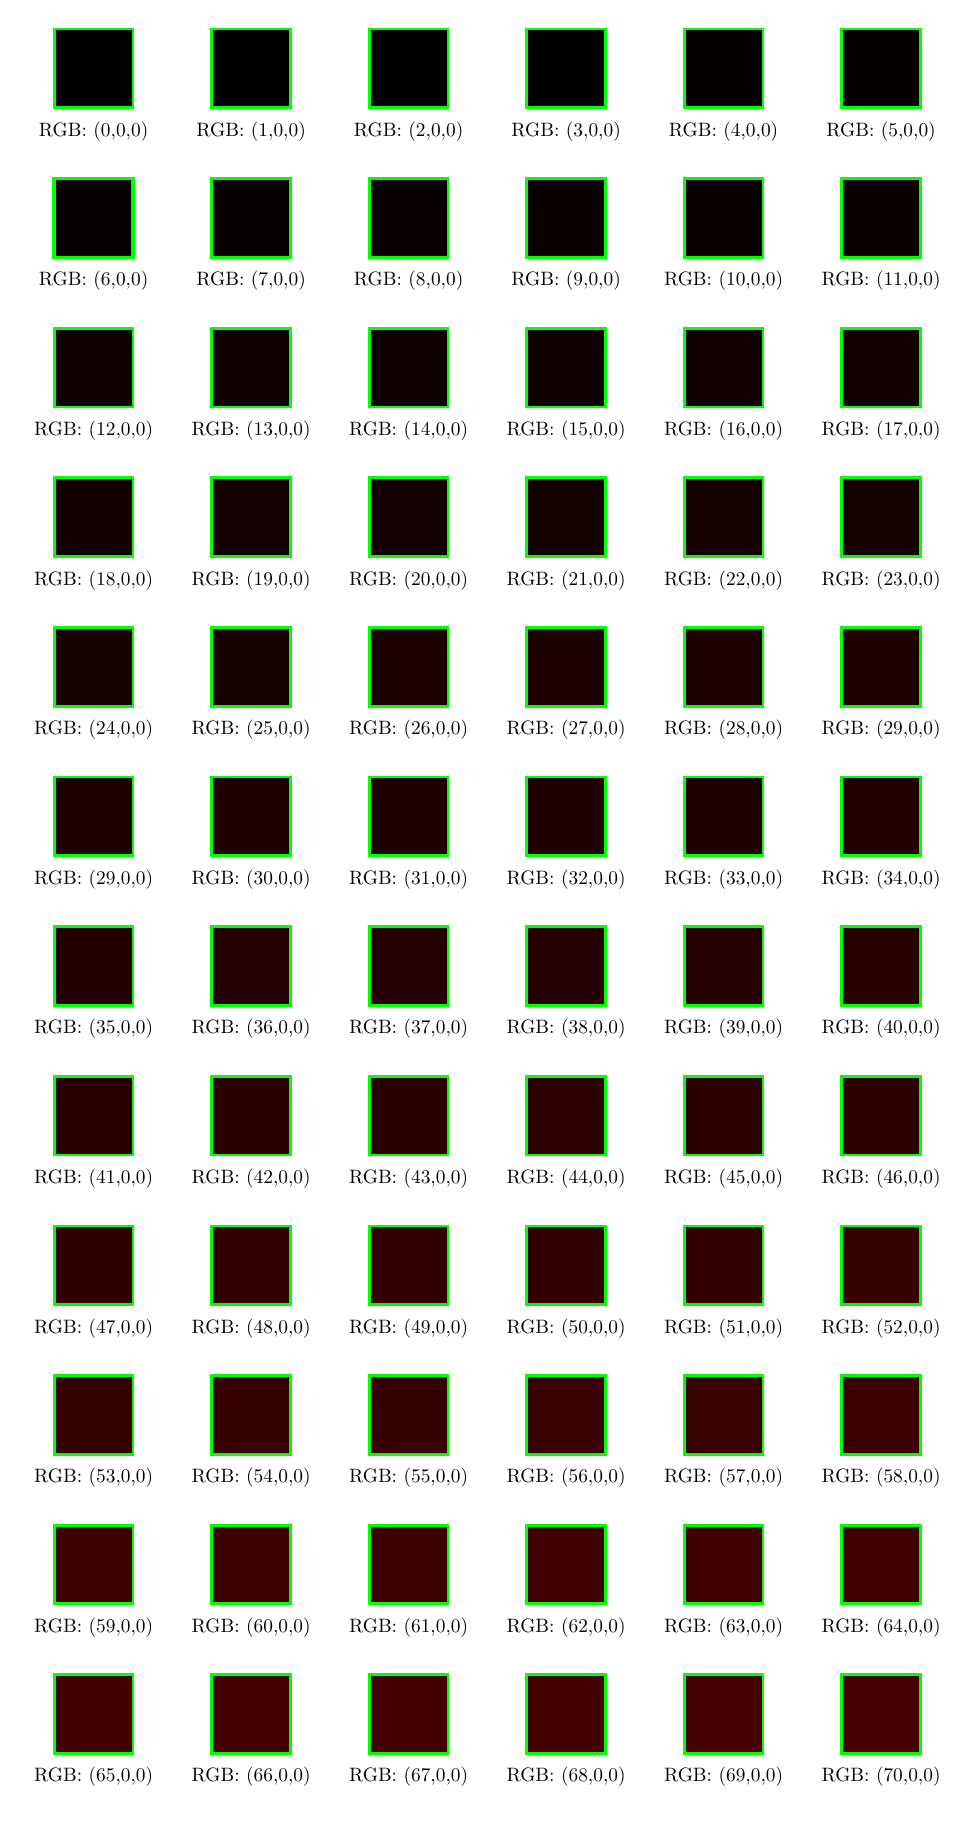
\begin{tikzpicture}

    \filldraw[draw=green,line width=1,fill=colorR0G0B0]
    (0,0) rectangle (1,1);

    \node[scale=0.7] at (0.5,-0.3) {RGB: (0,0,0)};



    \begin{scope}[xshift=2cm]

      \filldraw[draw=green,line width=1,fill=colorR1G0B0]
      (0,0) rectangle (1,1);

      \node[scale=0.7] at (0.5,-0.3) {RGB: (1,0,0)};

    \end{scope}



    \begin{scope}[xshift=4cm]

      \filldraw[draw=green,line width=1,fill=colorR2G0B0]
      (0,0) rectangle (1,1);

      \node[scale=0.7] at (0.5,-0.3) {RGB: (2,0,0)};

    \end{scope}



    \begin{scope}[xshift=6cm]

      \filldraw[draw=green,line width=1,fill=colorR3G0B0]
      (0,0) rectangle (1,1);

      \node[scale=0.7] at (0.5,-0.3) {RGB: (3,0,0)};

    \end{scope}



    \begin{scope}[xshift=8cm]

      \filldraw[draw=green,line width=1,fill=colorR4G0B0]
      (0,0) rectangle (1,1);

      \node[scale=0.7] at (0.5,-0.3) {RGB: (4,0,0)};

    \end{scope}



    \begin{scope}[xshift=10cm]

      \filldraw[draw=green,line width=1,fill=colorR5G0B0]
      (0,0) rectangle (1,1);

      \node[scale=0.7] at (0.5,-0.3) {RGB: (5,0,0)};

    \end{scope}





    \begin{scope}[yshift=-1.9cm]

      \filldraw[draw=green,line width=1.3,fill=colorR6G0B0]
      (0,0) rectangle (1,1);

      \node[scale=0.7] at (0.5,-0.3) {RGB: (6,0,0)};

    \end{scope}



    \begin{scope}[xshift=2cm,yshift=-1.9cm]

      \filldraw[draw=green,line width=1,fill=colorR7G0B0]
      (0,0) rectangle (1,1);

      \node[scale=0.7] at (0.5,-0.3) {RGB: (7,0,0)};

    \end{scope}



    \begin{scope}[xshift=4cm,yshift=-1.9cm]

      \filldraw[draw=green,line width=1,fill=colorR8G0B0]
      (0,0) rectangle (1,1);

      \node[scale=0.7] at (0.5,-0.3) {RGB: (8,0,0)};

    \end{scope}



    \begin{scope}[xshift=6cm,yshift=-1.9cm]

      \filldraw[draw=green,line width=1,fill=colorR9G0B0]
      (0,0) rectangle (1,1);

      \node[scale=0.7] at (0.5,-0.3) {RGB: (9,0,0)};

    \end{scope}



    \begin{scope}[xshift=8cm,yshift=-1.9cm]

      \filldraw[draw=green,line width=1,fill=colorR10G0B0]
      (0,0) rectangle (1,1);

      \node[scale=0.7] at (0.5,-0.3) {RGB: (10,0,0)};

    \end{scope}



    \begin{scope}[xshift=10cm,yshift=-1.9cm]

      \filldraw[draw=green,line width=1,fill=colorR11G0B0]
      (0,0) rectangle (1,1);

      \node[scale=0.7] at (0.5,-0.3) {RGB: (11,0,0)};

    \end{scope}





    \begin{scope}[yshift=-3.8cm]

      \filldraw[draw=green,line width=1,fill=colorR12G0B0]
      (0,0) rectangle (1,1);

      \node[scale=0.7] at (0.5,-0.3) {RGB: (12,0,0)};

    \end{scope}



    \begin{scope}[xshift=2cm,yshift=-3.8cm]

      \filldraw[draw=green,line width=1,fill=colorR13G0B0]
      (0,0) rectangle (1,1);

      \node[scale=0.7] at (0.5,-0.3) {RGB: (13,0,0)};

    \end{scope}



    \begin{scope}[xshift=4cm,yshift=-3.8cm]

      \filldraw[draw=green,line width=1,fill=colorR14G0B0]
      (0,0) rectangle (1,1);

      \node[scale=0.7] at (0.5,-0.3) {RGB: (14,0,0)};

    \end{scope}



    \begin{scope}[xshift=6cm,yshift=-3.8cm]

      \filldraw[draw=green,line width=1,fill=colorR15G0B0]
      (0,0) rectangle (1,1);

      \node[scale=0.7] at (0.5,-0.3) {RGB: (15,0,0)};

    \end{scope}



    \begin{scope}[xshift=8cm,yshift=-3.8cm]

      \filldraw[draw=green,line width=1,fill=colorR16G0B0]
      (0,0) rectangle (1,1);

      \node[scale=0.7] at (0.5,-0.3) {RGB: (16,0,0)};

    \end{scope}



    \begin{scope}[xshift=10cm,yshift=-3.8cm]

      \filldraw[draw=green,line width=1,fill=colorR17G0B0]
      (0,0) rectangle (1,1);

      \node[scale=0.7] at (0.5,-0.3) {RGB: (17,0,0)};

    \end{scope}





    \begin{scope}[yshift=-5.7cm]

      \filldraw[draw=green,line width=1,fill=colorR18G0B0]
      (0,0) rectangle (1,1);

      \node[scale=0.7] at (0.5,-0.3) {RGB: (18,0,0)};

    \end{scope}



    \begin{scope}[xshift=2cm,yshift=-5.7cm]

      \filldraw[draw=green,line width=1,fill=colorR19G0B0]
      (0,0) rectangle (1,1);

      \node[scale=0.7] at (0.5,-0.3) {RGB: (19,0,0)};

    \end{scope}



    \begin{scope}[xshift=4cm,yshift=-5.7cm]

      \filldraw[draw=green,line width=1,fill=colorR20G0B0]
      (0,0) rectangle (1,1);

      \node[scale=0.7] at (0.5,-0.3) {RGB: (20,0,0)};

    \end{scope}



    \begin{scope}[xshift=6cm,yshift=-5.7cm]

      \filldraw[draw=green,line width=1,fill=colorR21G0B0]
      (0,0) rectangle (1,1);

      \node[scale=0.7] at (0.5,-0.3) {RGB: (21,0,0)};

    \end{scope}



    \begin{scope}[xshift=8cm,yshift=-5.7cm]

      \filldraw[draw=green,line width=1,fill=colorR22G0B0]
      (0,0) rectangle (1,1);

      \node[scale=0.7] at (0.5,-0.3) {RGB: (22,0,0)};

    \end{scope}



    \begin{scope}[xshift=10cm,yshift=-5.7cm]

      \filldraw[draw=green,line width=1,fill=colorR23G0B0]
      (0,0) rectangle (1,1);

      \node[scale=0.7] at (0.5,-0.3) {RGB: (23,0,0)};

    \end{scope}





    \begin{scope}[yshift=-7.6cm]

      \filldraw[draw=green,line width=1,fill=colorR24G0B0]
      (0,0) rectangle (1,1);

      \node[scale=0.7] at (0.5,-0.3) {RGB: (24,0,0)};

    \end{scope}



    \begin{scope}[xshift=2cm,yshift=-7.6cm]

      \filldraw[draw=green,line width=1,fill=colorR25G0B0]
      (0,0) rectangle (1,1);

      \node[scale=0.7] at (0.5,-0.3) {RGB: (25,0,0)};

    \end{scope}



    \begin{scope}[xshift=4cm,yshift=-7.6cm]

      \filldraw[draw=green,line width=1,fill=colorR26G0B0]
      (0,0) rectangle (1,1);

      \node[scale=0.7] at (0.5,-0.3) {RGB: (26,0,0)};

    \end{scope}



    \begin{scope}[xshift=6cm,yshift=-7.6cm]

      \filldraw[draw=green,line width=1,fill=colorR27G0B0]
      (0,0) rectangle (1,1);

      \node[scale=0.7] at (0.5,-0.3) {RGB: (27,0,0)};

    \end{scope}



    \begin{scope}[xshift=8cm,yshift=-7.6cm]

      \filldraw[draw=green,line width=1,fill=colorR28G0B0]
      (0,0) rectangle (1,1);

      \node[scale=0.7] at (0.5,-0.3) {RGB: (28,0,0)};

    \end{scope}



    \begin{scope}[xshift=10cm,yshift=-7.6cm]

      \filldraw[draw=green,line width=1,fill=colorR29G0B0]
      (0,0) rectangle (1,1);

      \node[scale=0.7] at (0.5,-0.3) {RGB: (29,0,0)};

    \end{scope}





    \begin{scope}[yshift=-9.5cm]

      \filldraw[draw=green,line width=1,fill=colorR29G0B0]
      (0,0) rectangle (1,1);

      \node[scale=0.7] at (0.5,-0.3) {RGB: (29,0,0)};

    \end{scope}



    \begin{scope}[xshift=2cm,yshift=-9.5cm]

      \filldraw[draw=green,line width=1,fill=colorR30G0B0]
      (0,0) rectangle (1,1);

      \node[scale=0.7] at (0.5,-0.3) {RGB: (30,0,0)};

    \end{scope}



    \begin{scope}[xshift=4cm,yshift=-9.5cm]

      \filldraw[draw=green,line width=1,fill=colorR31G0B0]
      (0,0) rectangle (1,1);

      \node[scale=0.7] at (0.5,-0.3) {RGB: (31,0,0)};

    \end{scope}



    \begin{scope}[xshift=6cm,yshift=-9.5cm]

      \filldraw[draw=green,line width=1,fill=colorR32G0B0]
      (0,0) rectangle (1,1);

      \node[scale=0.7] at (0.5,-0.3) {RGB: (32,0,0)};

    \end{scope}



    \begin{scope}[xshift=8cm,yshift=-9.5cm]

      \filldraw[draw=green,line width=1,fill=colorR33G0B0]
      (0,0) rectangle (1,1);

      \node[scale=0.7] at (0.5,-0.3) {RGB: (33,0,0)};

    \end{scope}



    \begin{scope}[xshift=10cm,yshift=-9.5cm]

      \filldraw[draw=green,line width=1,fill=colorR34G0B0]
      (0,0) rectangle (1,1);

      \node[scale=0.7] at (0.5,-0.3) {RGB: (34,0,0)};

    \end{scope}





    \begin{scope}[yshift=-11.4cm]

      \filldraw[draw=green,line width=1,fill=colorR35G0B0]
      (0,0) rectangle (1,1);

      \node[scale=0.7] at (0.5,-0.3) {RGB: (35,0,0)};

    \end{scope}



    \begin{scope}[xshift=2cm,yshift=-11.4cm]

      \filldraw[draw=green,line width=1,fill=colorR36G0B0]
      (0,0) rectangle (1,1);

      \node[scale=0.7] at (0.5,-0.3) {RGB: (36,0,0)};

    \end{scope}



    \begin{scope}[xshift=4cm,yshift=-11.4cm]

      \filldraw[draw=green,line width=1,fill=colorR37G0B0]
      (0,0) rectangle (1,1);

      \node[scale=0.7] at (0.5,-0.3) {RGB: (37,0,0)};

    \end{scope}



    \begin{scope}[xshift=6cm,yshift=-11.4cm]

      \filldraw[draw=green,line width=1,fill=colorR38G0B0]
      (0,0) rectangle (1,1);

      \node[scale=0.7] at (0.5,-0.3) {RGB: (38,0,0)};

    \end{scope}



    \begin{scope}[xshift=8cm,yshift=-11.4cm]

      \filldraw[draw=green,line width=1,fill=colorR39G0B0]
      (0,0) rectangle (1,1);

      \node[scale=0.7] at (0.5,-0.3) {RGB: (39,0,0)};

    \end{scope}



    \begin{scope}[xshift=10cm,yshift=-11.4cm]

      \filldraw[draw=green,line width=1,fill=colorR40G0B0]
      (0,0) rectangle (1,1);

      \node[scale=0.7] at (0.5,-0.3) {RGB: (40,0,0)};

    \end{scope}





    \begin{scope}[yshift=-13.3cm]

      \filldraw[draw=green,line width=1,fill=colorR41G0B0]
      (0,0) rectangle (1,1);

      \node[scale=0.7] at (0.5,-0.3) {RGB: (41,0,0)};

    \end{scope}



    \begin{scope}[xshift=2cm,yshift=-13.3cm]

      \filldraw[draw=green,line width=1,fill=colorR42G0B0]
      (0,0) rectangle (1,1);

      \node[scale=0.7] at (0.5,-0.3) {RGB: (42,0,0)};

    \end{scope}



    \begin{scope}[xshift=4cm,yshift=-13.3cm]

      \filldraw[draw=green,line width=1,fill=colorR43G0B0]
      (0,0) rectangle (1,1);

      \node[scale=0.7] at (0.5,-0.3) {RGB: (43,0,0)};

    \end{scope}



    \begin{scope}[xshift=6cm,yshift=-13.3cm]

      \filldraw[draw=green,line width=1,fill=colorR44G0B0]
      (0,0) rectangle (1,1);

      \node[scale=0.7] at (0.5,-0.3) {RGB: (44,0,0)};

    \end{scope}



    \begin{scope}[xshift=8cm,yshift=-13.3cm]

      \filldraw[draw=green,line width=1,fill=colorR45G0B0]
      (0,0) rectangle (1,1);

      \node[scale=0.7] at (0.5,-0.3) {RGB: (45,0,0)};

    \end{scope}



    \begin{scope}[xshift=10cm,yshift=-13.3cm]

      \filldraw[draw=green,line width=1,fill=colorR46G0B0]
      (0,0) rectangle (1,1);

      \node[scale=0.7] at (0.5,-0.3) {RGB: (46,0,0)};

    \end{scope}





    \begin{scope}[yshift=-15.2cm]

      \filldraw[draw=green,line width=1,fill=colorR47G0B0]
      (0,0) rectangle (1,1);

      \node[scale=0.7] at (0.5,-0.3) {RGB: (47,0,0)};

    \end{scope}



    \begin{scope}[xshift=2cm,yshift=-15.2cm]

      \filldraw[draw=green,line width=1,fill=colorR48G0B0]
      (0,0) rectangle (1,1);

      \node[scale=0.7] at (0.5,-0.3) {RGB: (48,0,0)};

    \end{scope}



    \begin{scope}[xshift=4cm,yshift=-15.2cm]

      \filldraw[draw=green,line width=1,fill=colorR49G0B0]
      (0,0) rectangle (1,1);

      \node[scale=0.7] at (0.5,-0.3) {RGB: (49,0,0)};

    \end{scope}



    \begin{scope}[xshift=6cm,yshift=-15.2cm]

      \filldraw[draw=green,line width=1,fill=colorR50G0B0]
      (0,0) rectangle (1,1);

      \node[scale=0.7] at (0.5,-0.3) {RGB: (50,0,0)};

    \end{scope}



    \begin{scope}[xshift=8cm,yshift=-15.2cm]

      \filldraw[draw=green,line width=1,fill=colorR51G0B0]
      (0,0) rectangle (1,1);

      \node[scale=0.7] at (0.5,-0.3) {RGB: (51,0,0)};

    \end{scope}



    \begin{scope}[xshift=10cm,yshift=-15.2cm]

      \filldraw[draw=green,line width=1,fill=colorR52G0B0]
      (0,0) rectangle (1,1);

      \node[scale=0.7] at (0.5,-0.3) {RGB: (52,0,0)};

    \end{scope}





    \begin{scope}[yshift=-17.1cm]

      \filldraw[draw=green,line width=1,fill=colorR53G0B0]
      (0,0) rectangle (1,1);

      \node[scale=0.7] at (0.5,-0.3) {RGB: (53,0,0)};

    \end{scope}



    \begin{scope}[xshift=2cm,yshift=-17.1cm]

      \filldraw[draw=green,line width=1,fill=colorR54G0B0]
      (0,0) rectangle (1,1);

      \node[scale=0.7] at (0.5,-0.3) {RGB: (54,0,0)};

    \end{scope}



    \begin{scope}[xshift=4cm,yshift=-17.1cm]

      \filldraw[draw=green,line width=1,fill=colorR55G0B0]
      (0,0) rectangle (1,1);

      \node[scale=0.7] at (0.5,-0.3) {RGB: (55,0,0)};

    \end{scope}



    \begin{scope}[xshift=6cm,yshift=-17.1cm]

      \filldraw[draw=green,line width=1,fill=colorR56G0B0]
      (0,0) rectangle (1,1);

      \node[scale=0.7] at (0.5,-0.3) {RGB: (56,0,0)};

    \end{scope}



    \begin{scope}[xshift=8cm,yshift=-17.1cm]

      \filldraw[draw=green,line width=1,fill=colorR57G0B0]
      (0,0) rectangle (1,1);

      \node[scale=0.7] at (0.5,-0.3) {RGB: (57,0,0)};

    \end{scope}



    \begin{scope}[xshift=10cm,yshift=-17.1cm]

      \filldraw[draw=green,line width=1,fill=colorR58G0B0]
      (0,0) rectangle (1,1);

      \node[scale=0.7] at (0.5,-0.3) {RGB: (58,0,0)};

    \end{scope}





    \begin{scope}[yshift=-19cm]

      \filldraw[draw=green,line width=1,fill=colorR59G0B0]
      (0,0) rectangle (1,1);

      \node[scale=0.7] at (0.5,-0.3) {RGB: (59,0,0)};

    \end{scope}



    \begin{scope}[xshift=2cm,yshift=-19cm]

      \filldraw[draw=green,line width=1,fill=colorR60G0B0]
      (0,0) rectangle (1,1);

      \node[scale=0.7] at (0.5,-0.3) {RGB: (60,0,0)};

    \end{scope}



    \begin{scope}[xshift=4cm,yshift=-19cm]

      \filldraw[draw=green,line width=1,fill=colorR61G0B0]
      (0,0) rectangle (1,1);

      \node[scale=0.7] at (0.5,-0.3) {RGB: (61,0,0)};

    \end{scope}



    \begin{scope}[xshift=6cm,yshift=-19cm]

      \filldraw[draw=green,line width=1,fill=colorR62G0B0]
      (0,0) rectangle (1,1);

      \node[scale=0.7] at (0.5,-0.3) {RGB: (62,0,0)};

    \end{scope}



    \begin{scope}[xshift=8cm,yshift=-19cm]

      \filldraw[draw=green,line width=1,fill=colorR63G0B0]
      (0,0) rectangle (1,1);

      \node[scale=0.7] at (0.5,-0.3) {RGB: (63,0,0)};

    \end{scope}



    \begin{scope}[xshift=10cm,yshift=-19cm]

      \filldraw[draw=green,line width=1,fill=colorR64G0B0]
      (0,0) rectangle (1,1);

      \node[scale=0.7] at (0.5,-0.3) {RGB: (64,0,0)};

    \end{scope}





    \begin{scope}[yshift=-20.9cm]

      \filldraw[draw=green,line width=1,fill=colorR65G0B0]
      (0,0) rectangle (1,1);

      \node[scale=0.7] at (0.5,-0.3) {RGB: (65,0,0)};

    \end{scope}



    \begin{scope}[xshift=2cm,yshift=-20.9cm]

      \filldraw[draw=green,line width=1,fill=colorR66G0B0]
      (0,0) rectangle (1,1);

      \node[scale=0.7] at (0.5,-0.3) {RGB: (66,0,0)};

    \end{scope}



    \begin{scope}[xshift=4cm,yshift=-20.9cm]

      \filldraw[draw=green,line width=1,fill=colorR67G0B0]
      (0,0) rectangle (1,1);

      \node[scale=0.7] at (0.5,-0.3) {RGB: (67,0,0)};

    \end{scope}



    \begin{scope}[xshift=6cm,yshift=-20.9cm]

      \filldraw[draw=green,line width=1,fill=colorR68G0B0]
      (0,0) rectangle (1,1);

      \node[scale=0.7] at (0.5,-0.3) {RGB: (68,0,0)};

    \end{scope}



    \begin{scope}[xshift=8cm,yshift=-20.9cm]

      \filldraw[draw=green,line width=1,fill=colorR69G0B0]
      (0,0) rectangle (1,1);

      \node[scale=0.7] at (0.5,-0.3) {RGB: (69,0,0)};

    \end{scope}



    \begin{scope}[xshift=10cm,yshift=-20.9cm]

      \filldraw[draw=green,line width=1,fill=colorR70G0B0]
      (0,0) rectangle (1,1);

      \node[scale=0.7] at (0.5,-0.3) {RGB: (70,0,0)};

    \end{scope}

  \end{tikzpicture}

  \caption{Główne składowe kolorów w~systemie~RGB: $(0,0,0)$--$(70,0,0)$}



  \label{fig:Basic-colors-Part-01}

\end{figure}
% ##################





% ##################
\begin{figure}

  \centering


  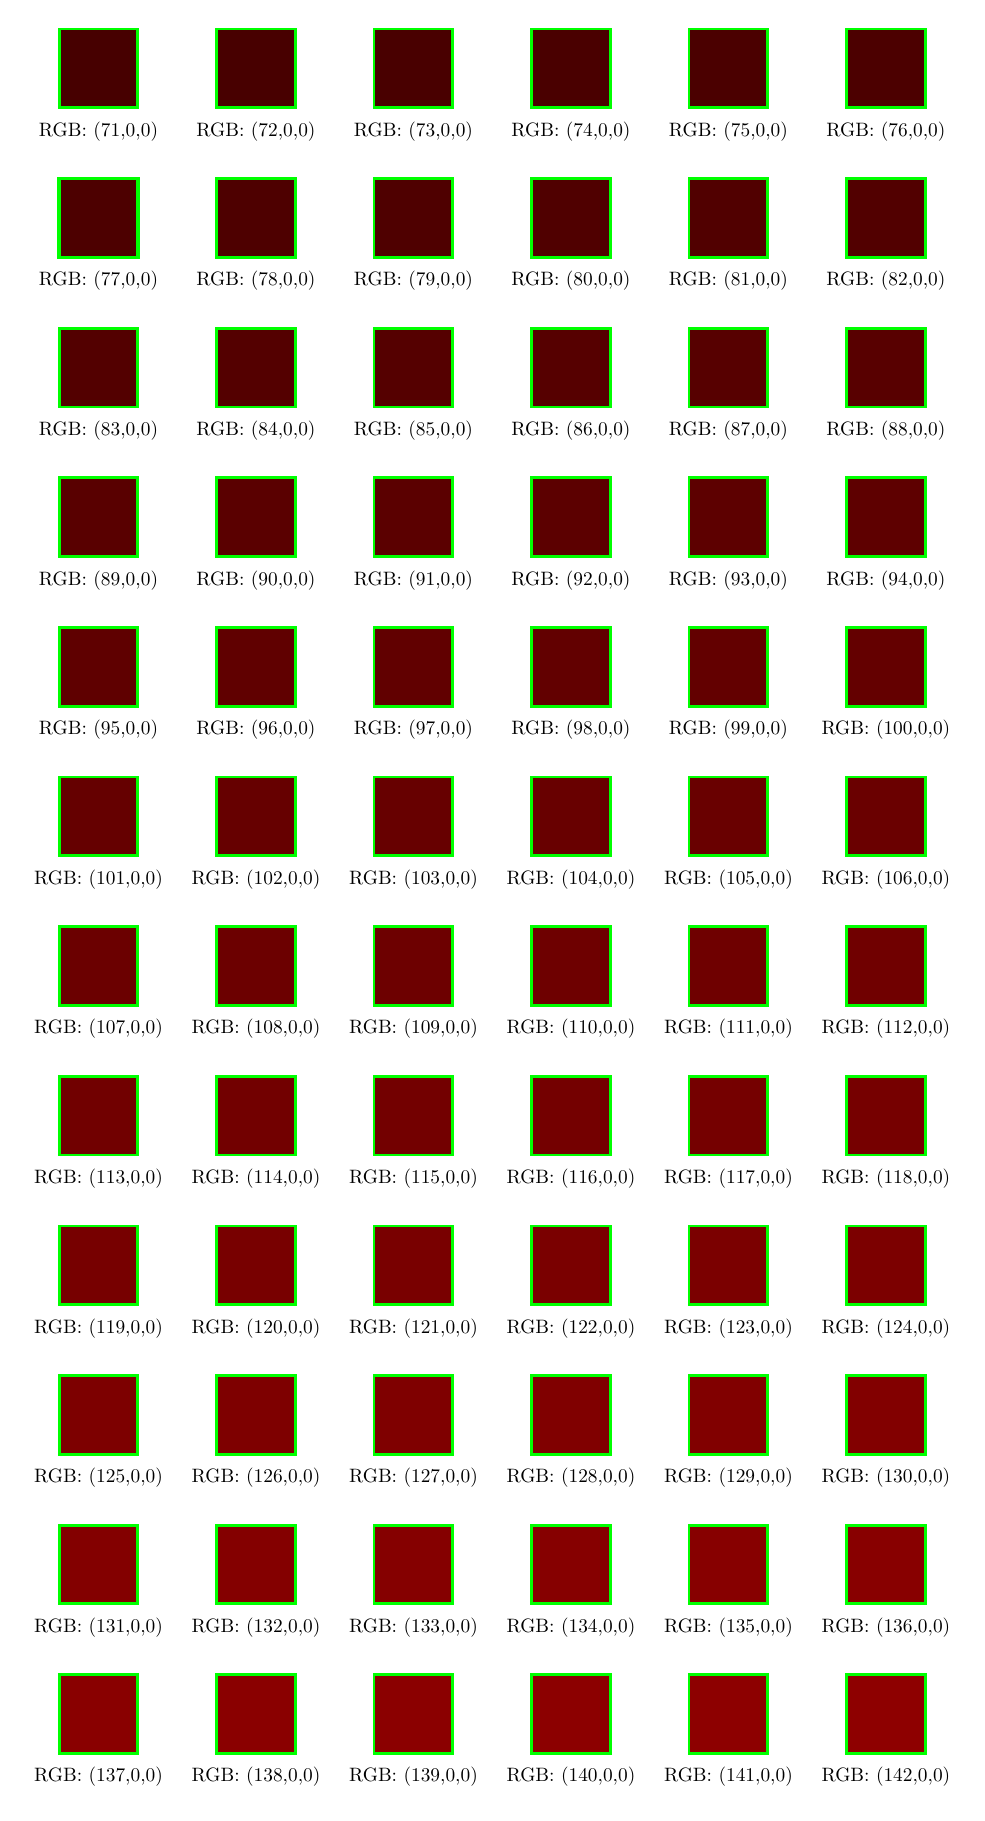
\begin{tikzpicture}

    \filldraw[draw=green,line width=1,fill=colorR71G0B0]
    (0,0) rectangle (1,1);

    \node[scale=0.7] at (0.5,-0.3) {RGB: (71,0,0)};



    \begin{scope}[xshift=2cm]

      \filldraw[draw=green,line width=1,fill=colorR72G0B0]
      (0,0) rectangle (1,1);

      \node[scale=0.7] at (0.5,-0.3) {RGB: (72,0,0)};

    \end{scope}



    \begin{scope}[xshift=4cm]

      \filldraw[draw=green,line width=1,fill=colorR73G0B0]
      (0,0) rectangle (1,1);

      \node[scale=0.7] at (0.5,-0.3) {RGB: (73,0,0)};

    \end{scope}



    \begin{scope}[xshift=6cm]

      \filldraw[draw=green,line width=1,fill=colorR74G0B0]
      (0,0) rectangle (1,1);

      \node[scale=0.7] at (0.5,-0.3) {RGB: (74,0,0)};

    \end{scope}



    \begin{scope}[xshift=8cm]

      \filldraw[draw=green,line width=1,fill=colorR75G0B0]
      (0,0) rectangle (1,1);

      \node[scale=0.7] at (0.5,-0.3) {RGB: (75,0,0)};

    \end{scope}



    \begin{scope}[xshift=10cm]

      \filldraw[draw=green,line width=1,fill=colorR76G0B0]
      (0,0) rectangle (1,1);

      \node[scale=0.7] at (0.5,-0.3) {RGB: (76,0,0)};

    \end{scope}





    \begin{scope}[yshift=-1.9cm]

      \filldraw[draw=green,line width=1.3,fill=colorR77G0B0]
      (0,0) rectangle (1,1);

      \node[scale=0.7] at (0.5,-0.3) {RGB: (77,0,0)};

    \end{scope}



    \begin{scope}[xshift=2cm,yshift=-1.9cm]

      \filldraw[draw=green,line width=1,fill=colorR78G0B0]
      (0,0) rectangle (1,1);

      \node[scale=0.7] at (0.5,-0.3) {RGB: (78,0,0)};

    \end{scope}



    \begin{scope}[xshift=4cm,yshift=-1.9cm]

      \filldraw[draw=green,line width=1,fill=colorR79G0B0]
      (0,0) rectangle (1,1);

      \node[scale=0.7] at (0.5,-0.3) {RGB: (79,0,0)};

    \end{scope}



    \begin{scope}[xshift=6cm,yshift=-1.9cm]

      \filldraw[draw=green,line width=1,fill=colorR80G0B0]
      (0,0) rectangle (1,1);

      \node[scale=0.7] at (0.5,-0.3) {RGB: (80,0,0)};

    \end{scope}



    \begin{scope}[xshift=8cm,yshift=-1.9cm]

      \filldraw[draw=green,line width=1,fill=colorR81G0B0]
      (0,0) rectangle (1,1);

      \node[scale=0.7] at (0.5,-0.3) {RGB: (81,0,0)};

    \end{scope}



    \begin{scope}[xshift=10cm,yshift=-1.9cm]

      \filldraw[draw=green,line width=1,fill=colorR82G0B0]
      (0,0) rectangle (1,1);

      \node[scale=0.7] at (0.5,-0.3) {RGB: (82,0,0)};

    \end{scope}





    \begin{scope}[yshift=-3.8cm]

      \filldraw[draw=green,line width=1,fill=colorR83G0B0]
      (0,0) rectangle (1,1);

      \node[scale=0.7] at (0.5,-0.3) {RGB: (83,0,0)};

    \end{scope}



    \begin{scope}[xshift=2cm,yshift=-3.8cm]

      \filldraw[draw=green,line width=1,fill=colorR84G0B0]
      (0,0) rectangle (1,1);

      \node[scale=0.7] at (0.5,-0.3) {RGB: (84,0,0)};

    \end{scope}



    \begin{scope}[xshift=4cm,yshift=-3.8cm]

      \filldraw[draw=green,line width=1,fill=colorR85G0B0]
      (0,0) rectangle (1,1);

      \node[scale=0.7] at (0.5,-0.3) {RGB: (85,0,0)};

    \end{scope}



    \begin{scope}[xshift=6cm,yshift=-3.8cm]

      \filldraw[draw=green,line width=1,fill=colorR86G0B0]
      (0,0) rectangle (1,1);

      \node[scale=0.7] at (0.5,-0.3) {RGB: (86,0,0)};

    \end{scope}



    \begin{scope}[xshift=8cm,yshift=-3.8cm]

      \filldraw[draw=green,line width=1,fill=colorR87G0B0]
      (0,0) rectangle (1,1);

      \node[scale=0.7] at (0.5,-0.3) {RGB: (87,0,0)};

    \end{scope}



    \begin{scope}[xshift=10cm,yshift=-3.8cm]

      \filldraw[draw=green,line width=1,fill=colorR88G0B0]
      (0,0) rectangle (1,1);

      \node[scale=0.7] at (0.5,-0.3) {RGB: (88,0,0)};

    \end{scope}





    \begin{scope}[yshift=-5.7cm]

      \filldraw[draw=green,line width=1,fill=colorR89G0B0]
      (0,0) rectangle (1,1);

      \node[scale=0.7] at (0.5,-0.3) {RGB: (89,0,0)};

    \end{scope}



    \begin{scope}[xshift=2cm,yshift=-5.7cm]

      \filldraw[draw=green,line width=1,fill=colorR90G0B0]
      (0,0) rectangle (1,1);

      \node[scale=0.7] at (0.5,-0.3) {RGB: (90,0,0)};

    \end{scope}



    \begin{scope}[xshift=4cm,yshift=-5.7cm]

      \filldraw[draw=green,line width=1,fill=colorR91G0B0]
      (0,0) rectangle (1,1);

      \node[scale=0.7] at (0.5,-0.3) {RGB: (91,0,0)};

    \end{scope}



    \begin{scope}[xshift=6cm,yshift=-5.7cm]

      \filldraw[draw=green,line width=1,fill=colorR92G0B0]
      (0,0) rectangle (1,1);

      \node[scale=0.7] at (0.5,-0.3) {RGB: (92,0,0)};

    \end{scope}



    \begin{scope}[xshift=8cm,yshift=-5.7cm]

      \filldraw[draw=green,line width=1,fill=colorR93G0B0]
      (0,0) rectangle (1,1);

      \node[scale=0.7] at (0.5,-0.3) {RGB: (93,0,0)};

    \end{scope}



    \begin{scope}[xshift=10cm,yshift=-5.7cm]

      \filldraw[draw=green,line width=1,fill=colorR94G0B0]
      (0,0) rectangle (1,1);

      \node[scale=0.7] at (0.5,-0.3) {RGB: (94,0,0)};

    \end{scope}





    \begin{scope}[yshift=-7.6cm]

      \filldraw[draw=green,line width=1,fill=colorR95G0B0]
      (0,0) rectangle (1,1);

      \node[scale=0.7] at (0.5,-0.3) {RGB: (95,0,0)};

    \end{scope}



    \begin{scope}[xshift=2cm,yshift=-7.6cm]

      \filldraw[draw=green,line width=1,fill=colorR96G0B0]
      (0,0) rectangle (1,1);

      \node[scale=0.7] at (0.5,-0.3) {RGB: (96,0,0)};

    \end{scope}



    \begin{scope}[xshift=4cm,yshift=-7.6cm]

      \filldraw[draw=green,line width=1,fill=colorR97G0B0]
      (0,0) rectangle (1,1);

      \node[scale=0.7] at (0.5,-0.3) {RGB: (97,0,0)};

    \end{scope}



    \begin{scope}[xshift=6cm,yshift=-7.6cm]

      \filldraw[draw=green,line width=1,fill=colorR98G0B0]
      (0,0) rectangle (1,1);

      \node[scale=0.7] at (0.5,-0.3) {RGB: (98,0,0)};

    \end{scope}



    \begin{scope}[xshift=8cm,yshift=-7.6cm]

      \filldraw[draw=green,line width=1,fill=colorR99G0B0]
      (0,0) rectangle (1,1);

      \node[scale=0.7] at (0.5,-0.3) {RGB: (99,0,0)};

    \end{scope}



    \begin{scope}[xshift=10cm,yshift=-7.6cm]

      \filldraw[draw=green,line width=1,fill=colorR100G0B0]
      (0,0) rectangle (1,1);

      \node[scale=0.7] at (0.5,-0.3) {RGB: (100,0,0)};

    \end{scope}





    \begin{scope}[yshift=-9.5cm]

      \filldraw[draw=green,line width=1,fill=colorR101G0B0]
      (0,0) rectangle (1,1);

      \node[scale=0.7] at (0.5,-0.3) {RGB: (101,0,0)};

    \end{scope}



    \begin{scope}[xshift=2cm,yshift=-9.5cm]

      \filldraw[draw=green,line width=1,fill=colorR102G0B0]
      (0,0) rectangle (1,1);

      \node[scale=0.7] at (0.5,-0.3) {RGB: (102,0,0)};

    \end{scope}



    \begin{scope}[xshift=4cm,yshift=-9.5cm]

      \filldraw[draw=green,line width=1,fill=colorR103G0B0]
      (0,0) rectangle (1,1);

      \node[scale=0.7] at (0.5,-0.3) {RGB: (103,0,0)};

    \end{scope}



    \begin{scope}[xshift=6cm,yshift=-9.5cm]

      \filldraw[draw=green,line width=1,fill=colorR104G0B0]
      (0,0) rectangle (1,1);

      \node[scale=0.7] at (0.5,-0.3) {RGB: (104,0,0)};

    \end{scope}



    \begin{scope}[xshift=8cm,yshift=-9.5cm]

      \filldraw[draw=green,line width=1,fill=colorR105G0B0]
      (0,0) rectangle (1,1);

      \node[scale=0.7] at (0.5,-0.3) {RGB: (105,0,0)};

    \end{scope}



    \begin{scope}[xshift=10cm,yshift=-9.5cm]

      \filldraw[draw=green,line width=1,fill=colorR106G0B0]
      (0,0) rectangle (1,1);

      \node[scale=0.7] at (0.5,-0.3) {RGB: (106,0,0)};

    \end{scope}





    \begin{scope}[yshift=-11.4cm]

      \filldraw[draw=green,line width=1,fill=colorR107G0B0]
      (0,0) rectangle (1,1);

      \node[scale=0.7] at (0.5,-0.3) {RGB: (107,0,0)};

    \end{scope}



    \begin{scope}[xshift=2cm,yshift=-11.4cm]

      \filldraw[draw=green,line width=1,fill=colorR108G0B0]
      (0,0) rectangle (1,1);

      \node[scale=0.7] at (0.5,-0.3) {RGB: (108,0,0)};

    \end{scope}



    \begin{scope}[xshift=4cm,yshift=-11.4cm]

      \filldraw[draw=green,line width=1,fill=colorR109G0B0]
      (0,0) rectangle (1,1);

      \node[scale=0.7] at (0.5,-0.3) {RGB: (109,0,0)};

    \end{scope}



    \begin{scope}[xshift=6cm,yshift=-11.4cm]

      \filldraw[draw=green,line width=1,fill=colorR110G0B0]
      (0,0) rectangle (1,1);

      \node[scale=0.7] at (0.5,-0.3) {RGB: (110,0,0)};

    \end{scope}



    \begin{scope}[xshift=8cm,yshift=-11.4cm]

      \filldraw[draw=green,line width=1,fill=colorR111G0B0]
      (0,0) rectangle (1,1);

      \node[scale=0.7] at (0.5,-0.3) {RGB: (111,0,0)};

    \end{scope}



    \begin{scope}[xshift=10cm,yshift=-11.4cm]

      \filldraw[draw=green,line width=1,fill=colorR112G0B0]
      (0,0) rectangle (1,1);

      \node[scale=0.7] at (0.5,-0.3) {RGB: (112,0,0)};

    \end{scope}





    \begin{scope}[yshift=-13.3cm]

      \filldraw[draw=green,line width=1,fill=colorR113G0B0]
      (0,0) rectangle (1,1);

      \node[scale=0.7] at (0.5,-0.3) {RGB: (113,0,0)};

    \end{scope}



    \begin{scope}[xshift=2cm,yshift=-13.3cm]

      \filldraw[draw=green,line width=1,fill=colorR114G0B0]
      (0,0) rectangle (1,1);

      \node[scale=0.7] at (0.5,-0.3) {RGB: (114,0,0)};

    \end{scope}



    \begin{scope}[xshift=4cm,yshift=-13.3cm]

      \filldraw[draw=green,line width=1,fill=colorR115G0B0]
      (0,0) rectangle (1,1);

      \node[scale=0.7] at (0.5,-0.3) {RGB: (115,0,0)};

    \end{scope}



    \begin{scope}[xshift=6cm,yshift=-13.3cm]

      \filldraw[draw=green,line width=1,fill=colorR116G0B0]
      (0,0) rectangle (1,1);

      \node[scale=0.7] at (0.5,-0.3) {RGB: (116,0,0)};

    \end{scope}



    \begin{scope}[xshift=8cm,yshift=-13.3cm]

      \filldraw[draw=green,line width=1,fill=colorR117G0B0]
      (0,0) rectangle (1,1);

      \node[scale=0.7] at (0.5,-0.3) {RGB: (117,0,0)};

    \end{scope}



    \begin{scope}[xshift=10cm,yshift=-13.3cm]

      \filldraw[draw=green,line width=1,fill=colorR118G0B0]
      (0,0) rectangle (1,1);

      \node[scale=0.7] at (0.5,-0.3) {RGB: (118,0,0)};

    \end{scope}





    \begin{scope}[yshift=-15.2cm]

      \filldraw[draw=green,line width=1,fill=colorR119G0B0]
      (0,0) rectangle (1,1);

      \node[scale=0.7] at (0.5,-0.3) {RGB: (119,0,0)};

    \end{scope}



    \begin{scope}[xshift=2cm,yshift=-15.2cm]

      \filldraw[draw=green,line width=1,fill=colorR120G0B0]
      (0,0) rectangle (1,1);

      \node[scale=0.7] at (0.5,-0.3) {RGB: (120,0,0)};

    \end{scope}



    \begin{scope}[xshift=4cm,yshift=-15.2cm]

      \filldraw[draw=green,line width=1,fill=colorR121G0B0]
      (0,0) rectangle (1,1);

      \node[scale=0.7] at (0.5,-0.3) {RGB: (121,0,0)};

    \end{scope}



    \begin{scope}[xshift=6cm,yshift=-15.2cm]

      \filldraw[draw=green,line width=1,fill=colorR122G0B0]
      (0,0) rectangle (1,1);

      \node[scale=0.7] at (0.5,-0.3) {RGB: (122,0,0)};

    \end{scope}



    \begin{scope}[xshift=8cm,yshift=-15.2cm]

      \filldraw[draw=green,line width=1,fill=colorR123G0B0]
      (0,0) rectangle (1,1);

      \node[scale=0.7] at (0.5,-0.3) {RGB: (123,0,0)};

    \end{scope}



    \begin{scope}[xshift=10cm,yshift=-15.2cm]

      \filldraw[draw=green,line width=1,fill=colorR124G0B0]
      (0,0) rectangle (1,1);

      \node[scale=0.7] at (0.5,-0.3) {RGB: (124,0,0)};

    \end{scope}





    \begin{scope}[yshift=-17.1cm]

      \filldraw[draw=green,line width=1,fill=colorR125G0B0]
      (0,0) rectangle (1,1);

      \node[scale=0.7] at (0.5,-0.3) {RGB: (125,0,0)};

    \end{scope}



    \begin{scope}[xshift=2cm,yshift=-17.1cm]

      \filldraw[draw=green,line width=1,fill=colorR126G0B0]
      (0,0) rectangle (1,1);

      \node[scale=0.7] at (0.5,-0.3) {RGB: (126,0,0)};

    \end{scope}



    \begin{scope}[xshift=4cm,yshift=-17.1cm]

      \filldraw[draw=green,line width=1,fill=colorR127G0B0]
      (0,0) rectangle (1,1);

      \node[scale=0.7] at (0.5,-0.3) {RGB: (127,0,0)};

    \end{scope}



    \begin{scope}[xshift=6cm,yshift=-17.1cm]

      \filldraw[draw=green,line width=1,fill=colorR128G0B0]
      (0,0) rectangle (1,1);

      \node[scale=0.7] at (0.5,-0.3) {RGB: (128,0,0)};

    \end{scope}



    \begin{scope}[xshift=8cm,yshift=-17.1cm]

      \filldraw[draw=green,line width=1,fill=colorR129G0B0]
      (0,0) rectangle (1,1);

      \node[scale=0.7] at (0.5,-0.3) {RGB: (129,0,0)};

    \end{scope}



    \begin{scope}[xshift=10cm,yshift=-17.1cm]

      \filldraw[draw=green,line width=1,fill=colorR130G0B0]
      (0,0) rectangle (1,1);

      \node[scale=0.7] at (0.5,-0.3) {RGB: (130,0,0)};

    \end{scope}





    \begin{scope}[yshift=-19cm]

      \filldraw[draw=green,line width=1,fill=colorR131G0B0]
      (0,0) rectangle (1,1);

      \node[scale=0.7] at (0.5,-0.3) {RGB: (131,0,0)};

    \end{scope}



    \begin{scope}[xshift=2cm,yshift=-19cm]

      \filldraw[draw=green,line width=1,fill=colorR132G0B0]
      (0,0) rectangle (1,1);

      \node[scale=0.7] at (0.5,-0.3) {RGB: (132,0,0)};

    \end{scope}



    \begin{scope}[xshift=4cm,yshift=-19cm]

      \filldraw[draw=green,line width=1,fill=colorR133G0B0]
      (0,0) rectangle (1,1);

      \node[scale=0.7] at (0.5,-0.3) {RGB: (133,0,0)};

    \end{scope}



    \begin{scope}[xshift=6cm,yshift=-19cm]

      \filldraw[draw=green,line width=1,fill=colorR134G0B0]
      (0,0) rectangle (1,1);

      \node[scale=0.7] at (0.5,-0.3) {RGB: (134,0,0)};

    \end{scope}



    \begin{scope}[xshift=8cm,yshift=-19cm]

      \filldraw[draw=green,line width=1,fill=colorR135G0B0]
      (0,0) rectangle (1,1);

      \node[scale=0.7] at (0.5,-0.3) {RGB: (135,0,0)};

    \end{scope}



    \begin{scope}[xshift=10cm,yshift=-19cm]

      \filldraw[draw=green,line width=1,fill=colorR136G0B0]
      (0,0) rectangle (1,1);

      \node[scale=0.7] at (0.5,-0.3) {RGB: (136,0,0)};

    \end{scope}





    \begin{scope}[yshift=-20.9cm]

      \filldraw[draw=green,line width=1,fill=colorR137G0B0]
      (0,0) rectangle (1,1);

      \node[scale=0.7] at (0.5,-0.3) {RGB: (137,0,0)};

    \end{scope}



    \begin{scope}[xshift=2cm,yshift=-20.9cm]

      \filldraw[draw=green,line width=1,fill=colorR138G0B0]
      (0,0) rectangle (1,1);

      \node[scale=0.7] at (0.5,-0.3) {RGB: (138,0,0)};

    \end{scope}



    \begin{scope}[xshift=4cm,yshift=-20.9cm]

      \filldraw[draw=green,line width=1,fill=colorR139G0B0]
      (0,0) rectangle (1,1);

      \node[scale=0.7] at (0.5,-0.3) {RGB: (139,0,0)};

    \end{scope}



    \begin{scope}[xshift=6cm,yshift=-20.9cm]

      \filldraw[draw=green,line width=1,fill=colorR140G0B0]
      (0,0) rectangle (1,1);

      \node[scale=0.7] at (0.5,-0.3) {RGB: (140,0,0)};

    \end{scope}



    \begin{scope}[xshift=8cm,yshift=-20.9cm]

      \filldraw[draw=green,line width=1,fill=colorR141G0B0]
      (0,0) rectangle (1,1);

      \node[scale=0.7] at (0.5,-0.3) {RGB: (141,0,0)};

    \end{scope}



    \begin{scope}[xshift=10cm,yshift=-20.9cm]

      \filldraw[draw=green,line width=1,fill=colorR142G0B0]
      (0,0) rectangle (1,1);

      \node[scale=0.7] at (0.5,-0.3) {RGB: (142,0,0)};

    \end{scope}

  \end{tikzpicture}

  \caption{Główne składowe kolorów w~systemie~RGB: $(70,0,0)$--$(142,0,0)$}



  \label{fig:Basic-colors-Part-02}

\end{figure}
% ##################





% ##################
\begin{figure}

  \centering


  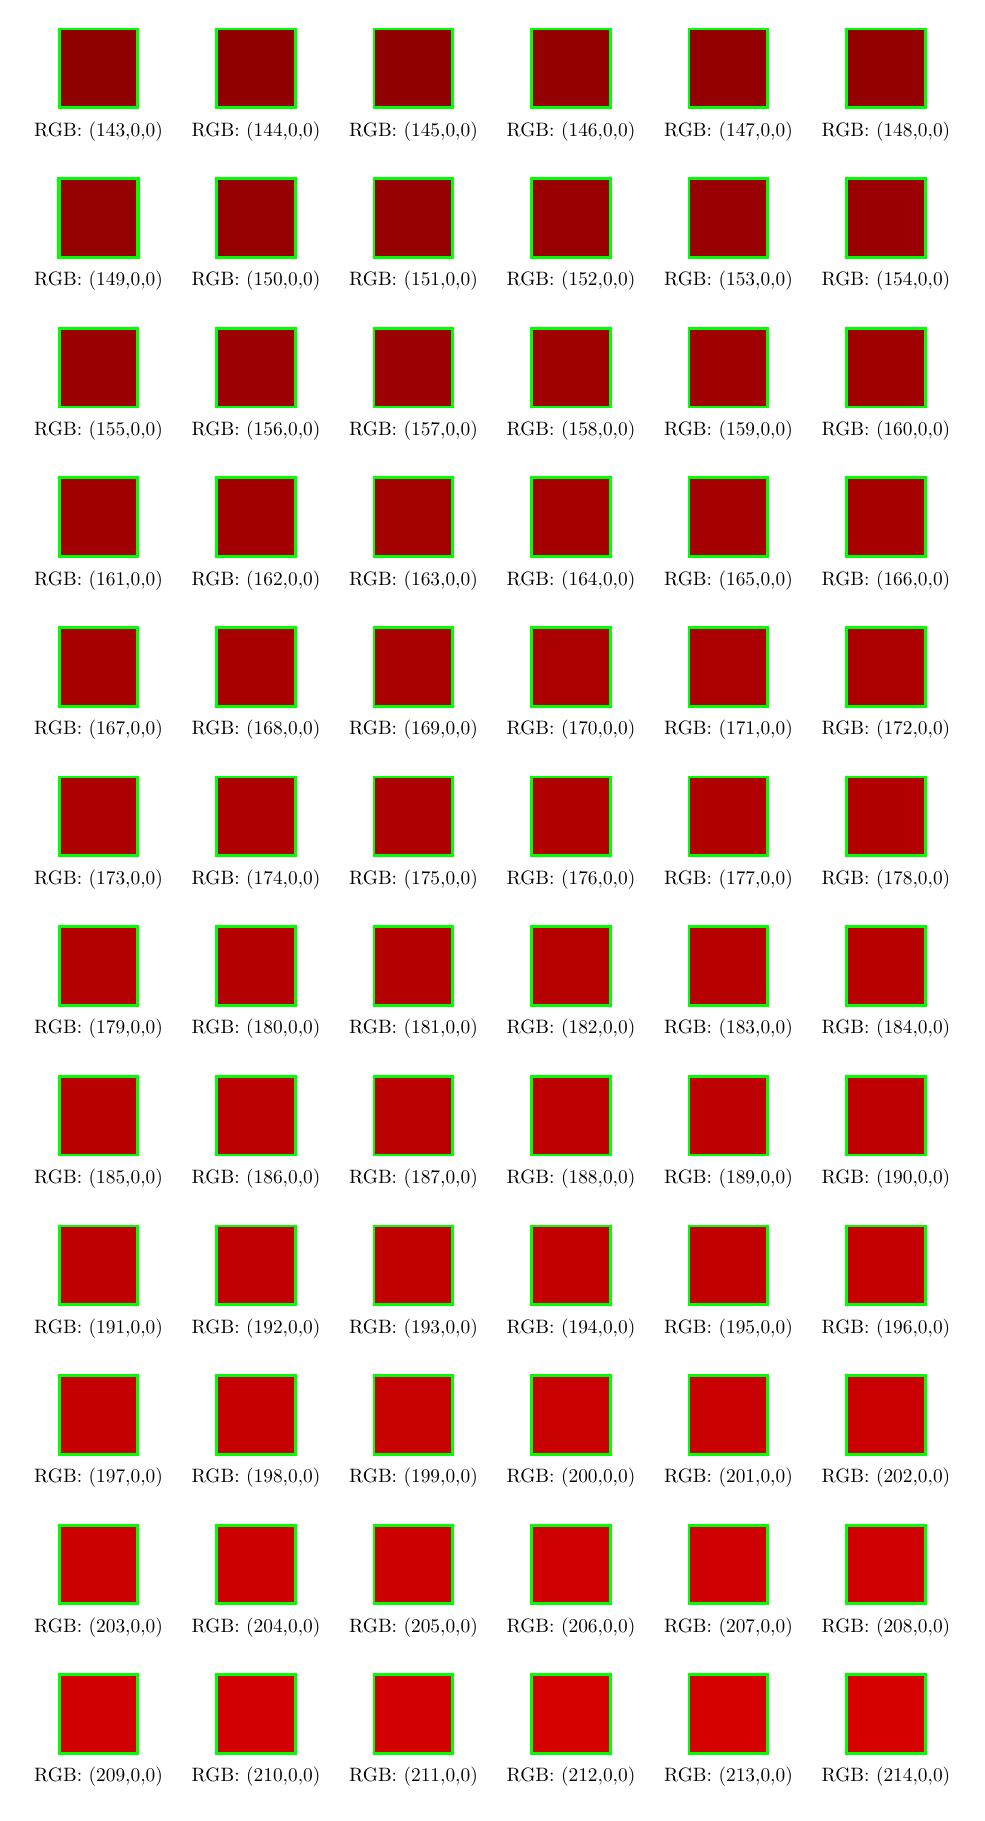
\begin{tikzpicture}

    \filldraw[draw=green,line width=1,fill=colorR143G0B0]
    (0,0) rectangle (1,1);

    \node[scale=0.7] at (0.5,-0.3) {RGB: (143,0,0)};



    \begin{scope}[xshift=2cm]

      \filldraw[draw=green,line width=1,fill=colorR144G0B0]
      (0,0) rectangle (1,1);

      \node[scale=0.7] at (0.5,-0.3) {RGB: (144,0,0)};

    \end{scope}



    \begin{scope}[xshift=4cm]

      \filldraw[draw=green,line width=1,fill=colorR145G0B0]
      (0,0) rectangle (1,1);

      \node[scale=0.7] at (0.5,-0.3) {RGB: (145,0,0)};

    \end{scope}



    \begin{scope}[xshift=6cm]

      \filldraw[draw=green,line width=1,fill=colorR146G0B0]
      (0,0) rectangle (1,1);

      \node[scale=0.7] at (0.5,-0.3) {RGB: (146,0,0)};

    \end{scope}



    \begin{scope}[xshift=8cm]

      \filldraw[draw=green,line width=1,fill=colorR147G0B0]
      (0,0) rectangle (1,1);

      \node[scale=0.7] at (0.5,-0.3) {RGB: (147,0,0)};

    \end{scope}



    \begin{scope}[xshift=10cm]

      \filldraw[draw=green,line width=1,fill=colorR148G0B0]
      (0,0) rectangle (1,1);

      \node[scale=0.7] at (0.5,-0.3) {RGB: (148,0,0)};

    \end{scope}





    \begin{scope}[yshift=-1.9cm]

      \filldraw[draw=green,line width=1.3,fill=colorR149G0B0]
      (0,0) rectangle (1,1);

      \node[scale=0.7] at (0.5,-0.3) {RGB: (149,0,0)};

    \end{scope}



    \begin{scope}[xshift=2cm,yshift=-1.9cm]

      \filldraw[draw=green,line width=1,fill=colorR150G0B0]
      (0,0) rectangle (1,1);

      \node[scale=0.7] at (0.5,-0.3) {RGB: (150,0,0)};

    \end{scope}



    \begin{scope}[xshift=4cm,yshift=-1.9cm]

      \filldraw[draw=green,line width=1,fill=colorR151G0B0]
      (0,0) rectangle (1,1);

      \node[scale=0.7] at (0.5,-0.3) {RGB: (151,0,0)};

    \end{scope}



    \begin{scope}[xshift=6cm,yshift=-1.9cm]

      \filldraw[draw=green,line width=1,fill=colorR152G0B0]
      (0,0) rectangle (1,1);

      \node[scale=0.7] at (0.5,-0.3) {RGB: (152,0,0)};

    \end{scope}



    \begin{scope}[xshift=8cm,yshift=-1.9cm]

      \filldraw[draw=green,line width=1,fill=colorR153G0B0]
      (0,0) rectangle (1,1);

      \node[scale=0.7] at (0.5,-0.3) {RGB: (153,0,0)};

    \end{scope}



    \begin{scope}[xshift=10cm,yshift=-1.9cm]

      \filldraw[draw=green,line width=1,fill=colorR154G0B0]
      (0,0) rectangle (1,1);

      \node[scale=0.7] at (0.5,-0.3) {RGB: (154,0,0)};

    \end{scope}





    \begin{scope}[yshift=-3.8cm]

      \filldraw[draw=green,line width=1,fill=colorR155G0B0]
      (0,0) rectangle (1,1);

      \node[scale=0.7] at (0.5,-0.3) {RGB: (155,0,0)};

    \end{scope}



    \begin{scope}[xshift=2cm,yshift=-3.8cm]

      \filldraw[draw=green,line width=1,fill=colorR156G0B0]
      (0,0) rectangle (1,1);

      \node[scale=0.7] at (0.5,-0.3) {RGB: (156,0,0)};

    \end{scope}



    \begin{scope}[xshift=4cm,yshift=-3.8cm]

      \filldraw[draw=green,line width=1,fill=colorR157G0B0]
      (0,0) rectangle (1,1);

      \node[scale=0.7] at (0.5,-0.3) {RGB: (157,0,0)};

    \end{scope}



    \begin{scope}[xshift=6cm,yshift=-3.8cm]

      \filldraw[draw=green,line width=1,fill=colorR158G0B0]
      (0,0) rectangle (1,1);

      \node[scale=0.7] at (0.5,-0.3) {RGB: (158,0,0)};

    \end{scope}



    \begin{scope}[xshift=8cm,yshift=-3.8cm]

      \filldraw[draw=green,line width=1,fill=colorR159G0B0]
      (0,0) rectangle (1,1);

      \node[scale=0.7] at (0.5,-0.3) {RGB: (159,0,0)};

    \end{scope}



    \begin{scope}[xshift=10cm,yshift=-3.8cm]

      \filldraw[draw=green,line width=1,fill=colorR160G0B0]
      (0,0) rectangle (1,1);

      \node[scale=0.7] at (0.5,-0.3) {RGB: (160,0,0)};

    \end{scope}





    \begin{scope}[yshift=-5.7cm]

      \filldraw[draw=green,line width=1,fill=colorR161G0B0]
      (0,0) rectangle (1,1);

      \node[scale=0.7] at (0.5,-0.3) {RGB: (161,0,0)};

    \end{scope}



    \begin{scope}[xshift=2cm,yshift=-5.7cm]

      \filldraw[draw=green,line width=1,fill=colorR162G0B0]
      (0,0) rectangle (1,1);

      \node[scale=0.7] at (0.5,-0.3) {RGB: (162,0,0)};

    \end{scope}



    \begin{scope}[xshift=4cm,yshift=-5.7cm]

      \filldraw[draw=green,line width=1,fill=colorR163G0B0]
      (0,0) rectangle (1,1);

      \node[scale=0.7] at (0.5,-0.3) {RGB: (163,0,0)};

    \end{scope}



    \begin{scope}[xshift=6cm,yshift=-5.7cm]

      \filldraw[draw=green,line width=1,fill=colorR164G0B0]
      (0,0) rectangle (1,1);

      \node[scale=0.7] at (0.5,-0.3) {RGB: (164,0,0)};

    \end{scope}



    \begin{scope}[xshift=8cm,yshift=-5.7cm]

      \filldraw[draw=green,line width=1,fill=colorR165G0B0]
      (0,0) rectangle (1,1);

      \node[scale=0.7] at (0.5,-0.3) {RGB: (165,0,0)};

    \end{scope}



    \begin{scope}[xshift=10cm,yshift=-5.7cm]

      \filldraw[draw=green,line width=1,fill=colorR166G0B0]
      (0,0) rectangle (1,1);

      \node[scale=0.7] at (0.5,-0.3) {RGB: (166,0,0)};

    \end{scope}





    \begin{scope}[yshift=-7.6cm]

      \filldraw[draw=green,line width=1,fill=colorR167G0B0]
      (0,0) rectangle (1,1);

      \node[scale=0.7] at (0.5,-0.3) {RGB: (167,0,0)};

    \end{scope}



    \begin{scope}[xshift=2cm,yshift=-7.6cm]

      \filldraw[draw=green,line width=1,fill=colorR168G0B0]
      (0,0) rectangle (1,1);

      \node[scale=0.7] at (0.5,-0.3) {RGB: (168,0,0)};

    \end{scope}



    \begin{scope}[xshift=4cm,yshift=-7.6cm]

      \filldraw[draw=green,line width=1,fill=colorR169G0B0]
      (0,0) rectangle (1,1);

      \node[scale=0.7] at (0.5,-0.3) {RGB: (169,0,0)};

    \end{scope}



    \begin{scope}[xshift=6cm,yshift=-7.6cm]

      \filldraw[draw=green,line width=1,fill=colorR170G0B0]
      (0,0) rectangle (1,1);

      \node[scale=0.7] at (0.5,-0.3) {RGB: (170,0,0)};

    \end{scope}



    \begin{scope}[xshift=8cm,yshift=-7.6cm]

      \filldraw[draw=green,line width=1,fill=colorR171G0B0]
      (0,0) rectangle (1,1);

      \node[scale=0.7] at (0.5,-0.3) {RGB: (171,0,0)};

    \end{scope}



    \begin{scope}[xshift=10cm,yshift=-7.6cm]

      \filldraw[draw=green,line width=1,fill=colorR172G0B0]
      (0,0) rectangle (1,1);

      \node[scale=0.7] at (0.5,-0.3) {RGB: (172,0,0)};

    \end{scope}





    \begin{scope}[yshift=-9.5cm]

      \filldraw[draw=green,line width=1,fill=colorR173G0B0]
      (0,0) rectangle (1,1);

      \node[scale=0.7] at (0.5,-0.3) {RGB: (173,0,0)};

    \end{scope}



    \begin{scope}[xshift=2cm,yshift=-9.5cm]

      \filldraw[draw=green,line width=1,fill=colorR174G0B0]
      (0,0) rectangle (1,1);

      \node[scale=0.7] at (0.5,-0.3) {RGB: (174,0,0)};

    \end{scope}



    \begin{scope}[xshift=4cm,yshift=-9.5cm]

      \filldraw[draw=green,line width=1,fill=colorR175G0B0]
      (0,0) rectangle (1,1);

      \node[scale=0.7] at (0.5,-0.3) {RGB: (175,0,0)};

    \end{scope}



    \begin{scope}[xshift=6cm,yshift=-9.5cm]

      \filldraw[draw=green,line width=1,fill=colorR176G0B0]
      (0,0) rectangle (1,1);

      \node[scale=0.7] at (0.5,-0.3) {RGB: (176,0,0)};

    \end{scope}



    \begin{scope}[xshift=8cm,yshift=-9.5cm]

      \filldraw[draw=green,line width=1,fill=colorR177G0B0]
      (0,0) rectangle (1,1);

      \node[scale=0.7] at (0.5,-0.3) {RGB: (177,0,0)};

    \end{scope}



    \begin{scope}[xshift=10cm,yshift=-9.5cm]

      \filldraw[draw=green,line width=1,fill=colorR178G0B0]
      (0,0) rectangle (1,1);

      \node[scale=0.7] at (0.5,-0.3) {RGB: (178,0,0)};

    \end{scope}





    \begin{scope}[yshift=-11.4cm]

      \filldraw[draw=green,line width=1,fill=colorR179G0B0]
      (0,0) rectangle (1,1);

      \node[scale=0.7] at (0.5,-0.3) {RGB: (179,0,0)};

    \end{scope}



    \begin{scope}[xshift=2cm,yshift=-11.4cm]

      \filldraw[draw=green,line width=1,fill=colorR180G0B0]
      (0,0) rectangle (1,1);

      \node[scale=0.7] at (0.5,-0.3) {RGB: (180,0,0)};

    \end{scope}



    \begin{scope}[xshift=4cm,yshift=-11.4cm]

      \filldraw[draw=green,line width=1,fill=colorR181G0B0]
      (0,0) rectangle (1,1);

      \node[scale=0.7] at (0.5,-0.3) {RGB: (181,0,0)};

    \end{scope}



    \begin{scope}[xshift=6cm,yshift=-11.4cm]

      \filldraw[draw=green,line width=1,fill=colorR182G0B0]
      (0,0) rectangle (1,1);

      \node[scale=0.7] at (0.5,-0.3) {RGB: (182,0,0)};

    \end{scope}



    \begin{scope}[xshift=8cm,yshift=-11.4cm]

      \filldraw[draw=green,line width=1,fill=colorR183G0B0]
      (0,0) rectangle (1,1);

      \node[scale=0.7] at (0.5,-0.3) {RGB: (183,0,0)};

    \end{scope}



    \begin{scope}[xshift=10cm,yshift=-11.4cm]

      \filldraw[draw=green,line width=1,fill=colorR184G0B0]
      (0,0) rectangle (1,1);

      \node[scale=0.7] at (0.5,-0.3) {RGB: (184,0,0)};

    \end{scope}





    \begin{scope}[yshift=-13.3cm]

      \filldraw[draw=green,line width=1,fill=colorR185G0B0]
      (0,0) rectangle (1,1);

      \node[scale=0.7] at (0.5,-0.3) {RGB: (185,0,0)};

    \end{scope}



    \begin{scope}[xshift=2cm,yshift=-13.3cm]

      \filldraw[draw=green,line width=1,fill=colorR186G0B0]
      (0,0) rectangle (1,1);

      \node[scale=0.7] at (0.5,-0.3) {RGB: (186,0,0)};

    \end{scope}



    \begin{scope}[xshift=4cm,yshift=-13.3cm]

      \filldraw[draw=green,line width=1,fill=colorR187G0B0]
      (0,0) rectangle (1,1);

      \node[scale=0.7] at (0.5,-0.3) {RGB: (187,0,0)};

    \end{scope}



    \begin{scope}[xshift=6cm,yshift=-13.3cm]

      \filldraw[draw=green,line width=1,fill=colorR188G0B0]
      (0,0) rectangle (1,1);

      \node[scale=0.7] at (0.5,-0.3) {RGB: (188,0,0)};

    \end{scope}



    \begin{scope}[xshift=8cm,yshift=-13.3cm]

      \filldraw[draw=green,line width=1,fill=colorR189G0B0]
      (0,0) rectangle (1,1);

      \node[scale=0.7] at (0.5,-0.3) {RGB: (189,0,0)};

    \end{scope}



    \begin{scope}[xshift=10cm,yshift=-13.3cm]

      \filldraw[draw=green,line width=1,fill=colorR190G0B0]
      (0,0) rectangle (1,1);

      \node[scale=0.7] at (0.5,-0.3) {RGB: (190,0,0)};

    \end{scope}





    \begin{scope}[yshift=-15.2cm]

      \filldraw[draw=green,line width=1,fill=colorR191G0B0]
      (0,0) rectangle (1,1);

      \node[scale=0.7] at (0.5,-0.3) {RGB: (191,0,0)};

    \end{scope}



    \begin{scope}[xshift=2cm,yshift=-15.2cm]

      \filldraw[draw=green,line width=1,fill=colorR192G0B0]
      (0,0) rectangle (1,1);

      \node[scale=0.7] at (0.5,-0.3) {RGB: (192,0,0)};

    \end{scope}



    \begin{scope}[xshift=4cm,yshift=-15.2cm]

      \filldraw[draw=green,line width=1,fill=colorR193G0B0]
      (0,0) rectangle (1,1);

      \node[scale=0.7] at (0.5,-0.3) {RGB: (193,0,0)};

    \end{scope}



    \begin{scope}[xshift=6cm,yshift=-15.2cm]

      \filldraw[draw=green,line width=1,fill=colorR194G0B0]
      (0,0) rectangle (1,1);

      \node[scale=0.7] at (0.5,-0.3) {RGB: (194,0,0)};

    \end{scope}



    \begin{scope}[xshift=8cm,yshift=-15.2cm]

      \filldraw[draw=green,line width=1,fill=colorR195G0B0]
      (0,0) rectangle (1,1);

      \node[scale=0.7] at (0.5,-0.3) {RGB: (195,0,0)};

    \end{scope}



    \begin{scope}[xshift=10cm,yshift=-15.2cm]

      \filldraw[draw=green,line width=1,fill=colorR196G0B0]
      (0,0) rectangle (1,1);

      \node[scale=0.7] at (0.5,-0.3) {RGB: (196,0,0)};

    \end{scope}





    \begin{scope}[yshift=-17.1cm]

      \filldraw[draw=green,line width=1,fill=colorR197G0B0]
      (0,0) rectangle (1,1);

      \node[scale=0.7] at (0.5,-0.3) {RGB: (197,0,0)};

    \end{scope}



    \begin{scope}[xshift=2cm,yshift=-17.1cm]

      \filldraw[draw=green,line width=1,fill=colorR198G0B0]
      (0,0) rectangle (1,1);

      \node[scale=0.7] at (0.5,-0.3) {RGB: (198,0,0)};

    \end{scope}



    \begin{scope}[xshift=4cm,yshift=-17.1cm]

      \filldraw[draw=green,line width=1,fill=colorR199G0B0]
      (0,0) rectangle (1,1);

      \node[scale=0.7] at (0.5,-0.3) {RGB: (199,0,0)};

    \end{scope}



    \begin{scope}[xshift=6cm,yshift=-17.1cm]

      \filldraw[draw=green,line width=1,fill=colorR200G0B0]
      (0,0) rectangle (1,1);

      \node[scale=0.7] at (0.5,-0.3) {RGB: (200,0,0)};

    \end{scope}



    \begin{scope}[xshift=8cm,yshift=-17.1cm]

      \filldraw[draw=green,line width=1,fill=colorR201G0B0]
      (0,0) rectangle (1,1);

      \node[scale=0.7] at (0.5,-0.3) {RGB: (201,0,0)};

    \end{scope}



    \begin{scope}[xshift=10cm,yshift=-17.1cm]

      \filldraw[draw=green,line width=1,fill=colorR202G0B0]
      (0,0) rectangle (1,1);

      \node[scale=0.7] at (0.5,-0.3) {RGB: (202,0,0)};

    \end{scope}





    \begin{scope}[yshift=-19cm]

      \filldraw[draw=green,line width=1,fill=colorR203G0B0]
      (0,0) rectangle (1,1);

      \node[scale=0.7] at (0.5,-0.3) {RGB: (203,0,0)};

    \end{scope}



    \begin{scope}[xshift=2cm,yshift=-19cm]

      \filldraw[draw=green,line width=1,fill=colorR204G0B0]
      (0,0) rectangle (1,1);

      \node[scale=0.7] at (0.5,-0.3) {RGB: (204,0,0)};

    \end{scope}



    \begin{scope}[xshift=4cm,yshift=-19cm]

      \filldraw[draw=green,line width=1,fill=colorR205G0B0]
      (0,0) rectangle (1,1);

      \node[scale=0.7] at (0.5,-0.3) {RGB: (205,0,0)};

    \end{scope}



    \begin{scope}[xshift=6cm,yshift=-19cm]

      \filldraw[draw=green,line width=1,fill=colorR206G0B0]
      (0,0) rectangle (1,1);

      \node[scale=0.7] at (0.5,-0.3) {RGB: (206,0,0)};

    \end{scope}



    \begin{scope}[xshift=8cm,yshift=-19cm]

      \filldraw[draw=green,line width=1,fill=colorR207G0B0]
      (0,0) rectangle (1,1);

      \node[scale=0.7] at (0.5,-0.3) {RGB: (207,0,0)};

    \end{scope}



    \begin{scope}[xshift=10cm,yshift=-19cm]

      \filldraw[draw=green,line width=1,fill=colorR208G0B0]
      (0,0) rectangle (1,1);

      \node[scale=0.7] at (0.5,-0.3) {RGB: (208,0,0)};

    \end{scope}





    \begin{scope}[yshift=-20.9cm]

      \filldraw[draw=green,line width=1,fill=colorR209G0B0]
      (0,0) rectangle (1,1);

      \node[scale=0.7] at (0.5,-0.3) {RGB: (209,0,0)};

    \end{scope}



    \begin{scope}[xshift=2cm,yshift=-20.9cm]

      \filldraw[draw=green,line width=1,fill=colorR210G0B0]
      (0,0) rectangle (1,1);

      \node[scale=0.7] at (0.5,-0.3) {RGB: (210,0,0)};

    \end{scope}



    \begin{scope}[xshift=4cm,yshift=-20.9cm]

      \filldraw[draw=green,line width=1,fill=colorR211G0B0]
      (0,0) rectangle (1,1);

      \node[scale=0.7] at (0.5,-0.3) {RGB: (211,0,0)};

    \end{scope}



    \begin{scope}[xshift=6cm,yshift=-20.9cm]

      \filldraw[draw=green,line width=1,fill=colorR212G0B0]
      (0,0) rectangle (1,1);

      \node[scale=0.7] at (0.5,-0.3) {RGB: (212,0,0)};

    \end{scope}



    \begin{scope}[xshift=8cm,yshift=-20.9cm]

      \filldraw[draw=green,line width=1,fill=colorR213G0B0]
      (0,0) rectangle (1,1);

      \node[scale=0.7] at (0.5,-0.3) {RGB: (213,0,0)};

    \end{scope}



    \begin{scope}[xshift=10cm,yshift=-20.9cm]

      \filldraw[draw=green,line width=1,fill=colorR214G0B0]
      (0,0) rectangle (1,1);

      \node[scale=0.7] at (0.5,-0.3) {RGB: (214,0,0)};

    \end{scope}

  \end{tikzpicture}

  \caption{Główne składowe kolorów w~systemie~RGB: $(143,0,0)$--$(214,0,0)$}



  \label{fig:Basic-colors-Part-03}

\end{figure}
% ##################





% ##################
\begin{figure}

  \centering


  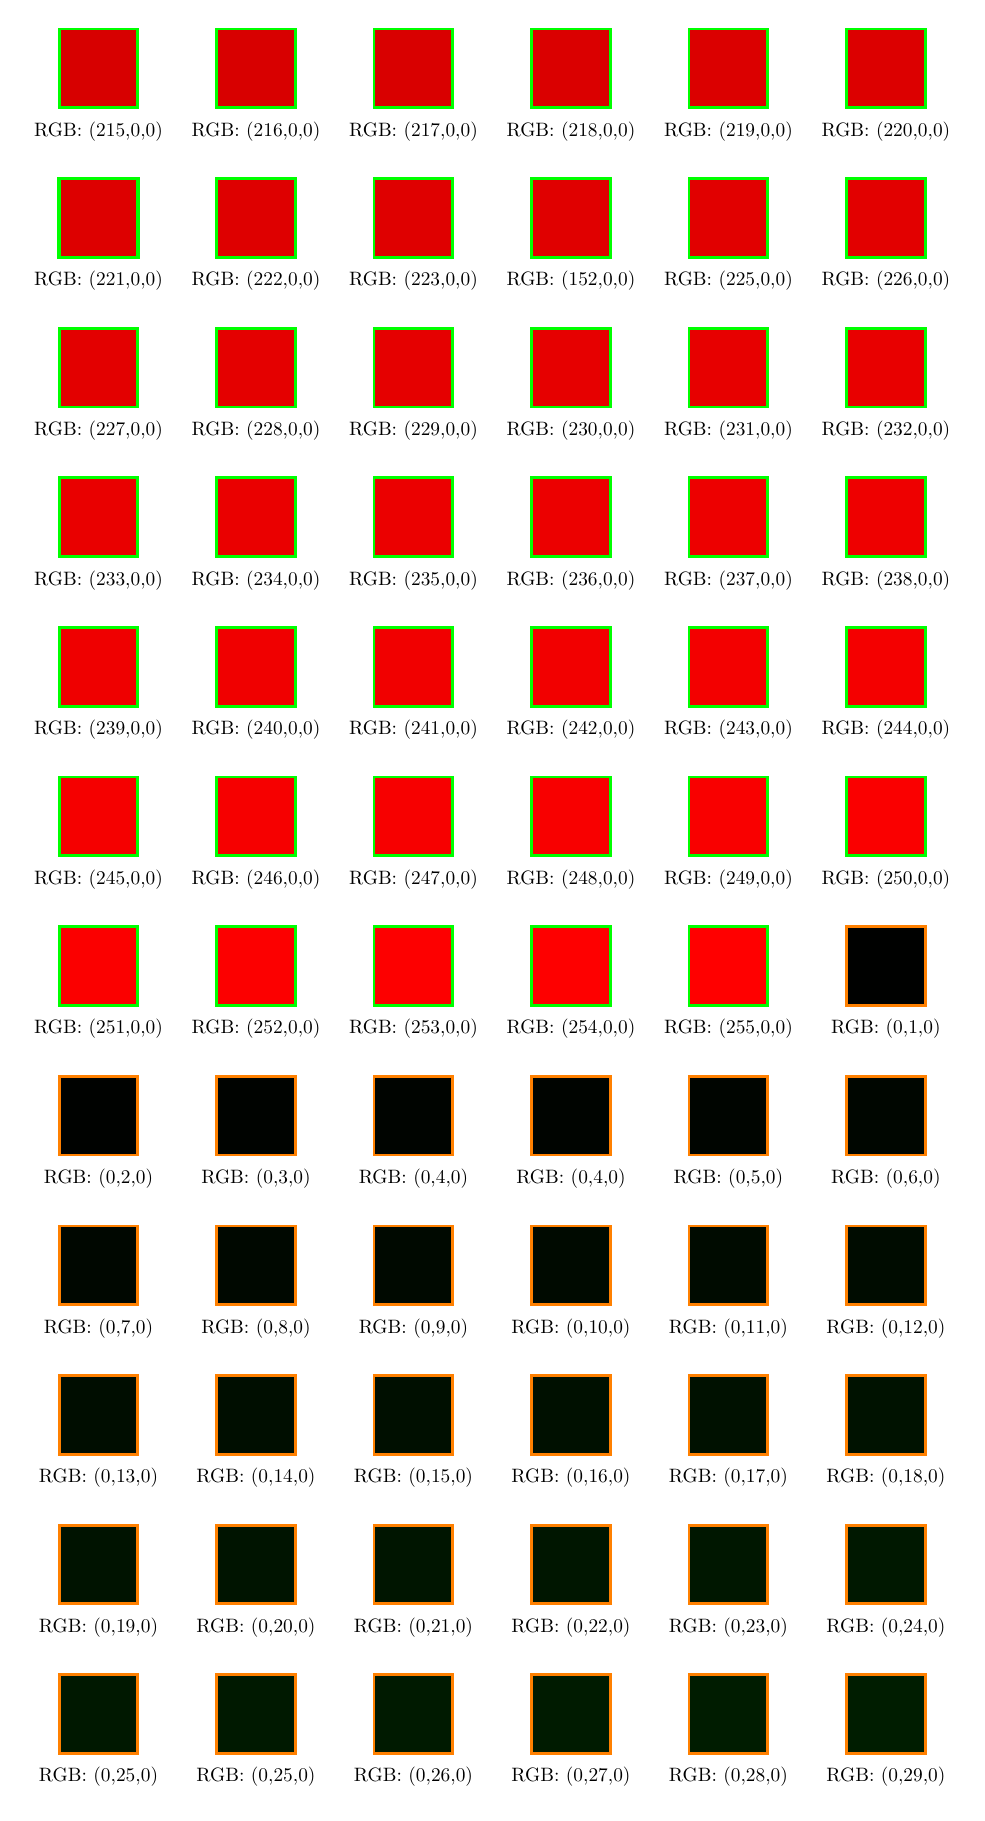
\begin{tikzpicture}

    \filldraw[draw=green,line width=1,fill=colorR215G0B0]
    (0,0) rectangle (1,1);

    \node[scale=0.7] at (0.5,-0.3) {RGB: (215,0,0)};



    \begin{scope}[xshift=2cm]

      \filldraw[draw=green,line width=1,fill=colorR216G0B0]
      (0,0) rectangle (1,1);

      \node[scale=0.7] at (0.5,-0.3) {RGB: (216,0,0)};

    \end{scope}



    \begin{scope}[xshift=4cm]

      \filldraw[draw=green,line width=1,fill=colorR217G0B0]
      (0,0) rectangle (1,1);

      \node[scale=0.7] at (0.5,-0.3) {RGB: (217,0,0)};

    \end{scope}



    \begin{scope}[xshift=6cm]

      \filldraw[draw=green,line width=1,fill=colorR218G0B0]
      (0,0) rectangle (1,1);

      \node[scale=0.7] at (0.5,-0.3) {RGB: (218,0,0)};

    \end{scope}



    \begin{scope}[xshift=8cm]

      \filldraw[draw=green,line width=1,fill=colorR219G0B0]
      (0,0) rectangle (1,1);

      \node[scale=0.7] at (0.5,-0.3) {RGB: (219,0,0)};

    \end{scope}



    \begin{scope}[xshift=10cm]

      \filldraw[draw=green,line width=1,fill=colorR220G0B0]
      (0,0) rectangle (1,1);

      \node[scale=0.7] at (0.5,-0.3) {RGB: (220,0,0)};

    \end{scope}





    \begin{scope}[yshift=-1.9cm]

      \filldraw[draw=green,line width=1.3,fill=colorR221G0B0]
      (0,0) rectangle (1,1);

      \node[scale=0.7] at (0.5,-0.3) {RGB: (221,0,0)};

    \end{scope}



    \begin{scope}[xshift=2cm,yshift=-1.9cm]

      \filldraw[draw=green,line width=1,fill=colorR222G0B0]
      (0,0) rectangle (1,1);

      \node[scale=0.7] at (0.5,-0.3) {RGB: (222,0,0)};

    \end{scope}



    \begin{scope}[xshift=4cm,yshift=-1.9cm]

      \filldraw[draw=green,line width=1,fill=colorR223G0B0]
      (0,0) rectangle (1,1);

      \node[scale=0.7] at (0.5,-0.3) {RGB: (223,0,0)};

    \end{scope}



    \begin{scope}[xshift=6cm,yshift=-1.9cm]

      \filldraw[draw=green,line width=1,fill=colorR224G0B0]
      (0,0) rectangle (1,1);

      \node[scale=0.7] at (0.5,-0.3) {RGB: (152,0,0)};

    \end{scope}



    \begin{scope}[xshift=8cm,yshift=-1.9cm]

      \filldraw[draw=green,line width=1,fill=colorR225G0B0]
      (0,0) rectangle (1,1);

      \node[scale=0.7] at (0.5,-0.3) {RGB: (225,0,0)};

    \end{scope}



    \begin{scope}[xshift=10cm,yshift=-1.9cm]

      \filldraw[draw=green,line width=1,fill=colorR226G0B0]
      (0,0) rectangle (1,1);

      \node[scale=0.7] at (0.5,-0.3) {RGB: (226,0,0)};

    \end{scope}





    \begin{scope}[yshift=-3.8cm]

      \filldraw[draw=green,line width=1,fill=colorR227G0B0]
      (0,0) rectangle (1,1);

      \node[scale=0.7] at (0.5,-0.3) {RGB: (227,0,0)};

    \end{scope}



    \begin{scope}[xshift=2cm,yshift=-3.8cm]

      \filldraw[draw=green,line width=1,fill=colorR228G0B0]
      (0,0) rectangle (1,1);

      \node[scale=0.7] at (0.5,-0.3) {RGB: (228,0,0)};

    \end{scope}



    \begin{scope}[xshift=4cm,yshift=-3.8cm]

      \filldraw[draw=green,line width=1,fill=colorR229G0B0]
      (0,0) rectangle (1,1);

      \node[scale=0.7] at (0.5,-0.3) {RGB: (229,0,0)};

    \end{scope}



    \begin{scope}[xshift=6cm,yshift=-3.8cm]

      \filldraw[draw=green,line width=1,fill=colorR230G0B0]
      (0,0) rectangle (1,1);

      \node[scale=0.7] at (0.5,-0.3) {RGB: (230,0,0)};

    \end{scope}



    \begin{scope}[xshift=8cm,yshift=-3.8cm]

      \filldraw[draw=green,line width=1,fill=colorR231G0B0]
      (0,0) rectangle (1,1);

      \node[scale=0.7] at (0.5,-0.3) {RGB: (231,0,0)};

    \end{scope}



    \begin{scope}[xshift=10cm,yshift=-3.8cm]

      \filldraw[draw=green,line width=1,fill=colorR232G0B0]
      (0,0) rectangle (1,1);

      \node[scale=0.7] at (0.5,-0.3) {RGB: (232,0,0)};

    \end{scope}





    \begin{scope}[yshift=-5.7cm]

      \filldraw[draw=green,line width=1,fill=colorR233G0B0]
      (0,0) rectangle (1,1);

      \node[scale=0.7] at (0.5,-0.3) {RGB: (233,0,0)};

    \end{scope}



    \begin{scope}[xshift=2cm,yshift=-5.7cm]

      \filldraw[draw=green,line width=1,fill=colorR234G0B0]
      (0,0) rectangle (1,1);

      \node[scale=0.7] at (0.5,-0.3) {RGB: (234,0,0)};

    \end{scope}



    \begin{scope}[xshift=4cm,yshift=-5.7cm]

      \filldraw[draw=green,line width=1,fill=colorR235G0B0]
      (0,0) rectangle (1,1);

      \node[scale=0.7] at (0.5,-0.3) {RGB: (235,0,0)};

    \end{scope}



    \begin{scope}[xshift=6cm,yshift=-5.7cm]

      \filldraw[draw=green,line width=1,fill=colorR236G0B0]
      (0,0) rectangle (1,1);

      \node[scale=0.7] at (0.5,-0.3) {RGB: (236,0,0)};

    \end{scope}



    \begin{scope}[xshift=8cm,yshift=-5.7cm]

      \filldraw[draw=green,line width=1,fill=colorR237G0B0]
      (0,0) rectangle (1,1);

      \node[scale=0.7] at (0.5,-0.3) {RGB: (237,0,0)};

    \end{scope}



    \begin{scope}[xshift=10cm,yshift=-5.7cm]

      \filldraw[draw=green,line width=1,fill=colorR238G0B0]
      (0,0) rectangle (1,1);

      \node[scale=0.7] at (0.5,-0.3) {RGB: (238,0,0)};

    \end{scope}





    \begin{scope}[yshift=-7.6cm]

      \filldraw[draw=green,line width=1,fill=colorR239G0B0]
      (0,0) rectangle (1,1);

      \node[scale=0.7] at (0.5,-0.3) {RGB: (239,0,0)};

    \end{scope}



    \begin{scope}[xshift=2cm,yshift=-7.6cm]

      \filldraw[draw=green,line width=1,fill=colorR240G0B0]
      (0,0) rectangle (1,1);

      \node[scale=0.7] at (0.5,-0.3) {RGB: (240,0,0)};

    \end{scope}



    \begin{scope}[xshift=4cm,yshift=-7.6cm]

      \filldraw[draw=green,line width=1,fill=colorR241G0B0]
      (0,0) rectangle (1,1);

      \node[scale=0.7] at (0.5,-0.3) {RGB: (241,0,0)};

    \end{scope}



    \begin{scope}[xshift=6cm,yshift=-7.6cm]

      \filldraw[draw=green,line width=1,fill=colorR242G0B0]
      (0,0) rectangle (1,1);

      \node[scale=0.7] at (0.5,-0.3) {RGB: (242,0,0)};

    \end{scope}



    \begin{scope}[xshift=8cm,yshift=-7.6cm]

      \filldraw[draw=green,line width=1,fill=colorR243G0B0]
      (0,0) rectangle (1,1);

      \node[scale=0.7] at (0.5,-0.3) {RGB: (243,0,0)};

    \end{scope}



    \begin{scope}[xshift=10cm,yshift=-7.6cm]

      \filldraw[draw=green,line width=1,fill=colorR244G0B0]
      (0,0) rectangle (1,1);

      \node[scale=0.7] at (0.5,-0.3) {RGB: (244,0,0)};

    \end{scope}





    \begin{scope}[yshift=-9.5cm]

      \filldraw[draw=green,line width=1,fill=colorR245G0B0]
      (0,0) rectangle (1,1);

      \node[scale=0.7] at (0.5,-0.3) {RGB: (245,0,0)};

    \end{scope}



    \begin{scope}[xshift=2cm,yshift=-9.5cm]

      \filldraw[draw=green,line width=1,fill=colorR246G0B0]
      (0,0) rectangle (1,1);

      \node[scale=0.7] at (0.5,-0.3) {RGB: (246,0,0)};

    \end{scope}



    \begin{scope}[xshift=4cm,yshift=-9.5cm]

      \filldraw[draw=green,line width=1,fill=colorR247G0B0]
      (0,0) rectangle (1,1);

      \node[scale=0.7] at (0.5,-0.3) {RGB: (247,0,0)};

    \end{scope}



    \begin{scope}[xshift=6cm,yshift=-9.5cm]

      \filldraw[draw=green,line width=1,fill=colorR248G0B0]
      (0,0) rectangle (1,1);

      \node[scale=0.7] at (0.5,-0.3) {RGB: (248,0,0)};

    \end{scope}



    \begin{scope}[xshift=8cm,yshift=-9.5cm]

      \filldraw[draw=green,line width=1,fill=colorR249G0B0]
      (0,0) rectangle (1,1);

      \node[scale=0.7] at (0.5,-0.3) {RGB: (249,0,0)};

    \end{scope}



    \begin{scope}[xshift=10cm,yshift=-9.5cm]

      \filldraw[draw=green,line width=1,fill=colorR250G0B0]
      (0,0) rectangle (1,1);

      \node[scale=0.7] at (0.5,-0.3) {RGB: (250,0,0)};

    \end{scope}





    \begin{scope}[yshift=-11.4cm]

      \filldraw[draw=green,line width=1,fill=colorR251G0B0]
      (0,0) rectangle (1,1);

      \node[scale=0.7] at (0.5,-0.3) {RGB: (251,0,0)};

    \end{scope}



    \begin{scope}[xshift=2cm,yshift=-11.4cm]

      \filldraw[draw=green,line width=1,fill=colorR252G0B0]
      (0,0) rectangle (1,1);

      \node[scale=0.7] at (0.5,-0.3) {RGB: (252,0,0)};

    \end{scope}



    \begin{scope}[xshift=4cm,yshift=-11.4cm]

      \filldraw[draw=green,line width=1,fill=colorR253G0B0]
      (0,0) rectangle (1,1);

      \node[scale=0.7] at (0.5,-0.3) {RGB: (253,0,0)};

    \end{scope}



    \begin{scope}[xshift=6cm,yshift=-11.4cm]

      \filldraw[draw=green,line width=1,fill=colorR254G0B0]
      (0,0) rectangle (1,1);

      \node[scale=0.7] at (0.5,-0.3) {RGB: (254,0,0)};

    \end{scope}



    \begin{scope}[xshift=8cm,yshift=-11.4cm]

      \filldraw[draw=green,line width=1,fill=colorR255G0B0]
      (0,0) rectangle (1,1);

      \node[scale=0.7] at (0.5,-0.3) {RGB: (255,0,0)};

    \end{scope}



    \begin{scope}[xshift=10cm,yshift=-11.4cm]

      \filldraw[draw=orange,line width=1,fill=colorR0G1B0]
      (0,0) rectangle (1,1);

      \node[scale=0.7] at (0.5,-0.3) {RGB: (0,1,0)};

    \end{scope}





    \begin{scope}[yshift=-13.3cm]

      \filldraw[draw=orange,line width=1,fill=colorR0G2B0]
      (0,0) rectangle (1,1);

      \node[scale=0.7] at (0.5,-0.3) {RGB: (0,2,0)};

    \end{scope}



    \begin{scope}[xshift=2cm,yshift=-13.3cm]

      \filldraw[draw=orange,line width=1,fill=colorR0G3B0]
      (0,0) rectangle (1,1);

      \node[scale=0.7] at (0.5,-0.3) {RGB: (0,3,0)};

    \end{scope}



    \begin{scope}[xshift=4cm,yshift=-13.3cm]

      \filldraw[draw=orange,line width=1,fill=colorR0G4B0]
      (0,0) rectangle (1,1);

      \node[scale=0.7] at (0.5,-0.3) {RGB: (0,4,0)};

    \end{scope}



    \begin{scope}[xshift=6cm,yshift=-13.3cm]

      \filldraw[draw=orange,line width=1,fill=colorR0G4B0]
      (0,0) rectangle (1,1);

      \node[scale=0.7] at (0.5,-0.3) {RGB: (0,4,0)};

    \end{scope}



    \begin{scope}[xshift=8cm,yshift=-13.3cm]

      \filldraw[draw=orange,line width=1,fill=colorR0G5B0]
      (0,0) rectangle (1,1);

      \node[scale=0.7] at (0.5,-0.3) {RGB: (0,5,0)};

    \end{scope}



    \begin{scope}[xshift=10cm,yshift=-13.3cm]

      \filldraw[draw=orange,line width=1,fill=colorR0G6B0]
      (0,0) rectangle (1,1);

      \node[scale=0.7] at (0.5,-0.3) {RGB: (0,6,0)};

    \end{scope}





    \begin{scope}[yshift=-15.2cm]

      \filldraw[draw=orange,line width=1,fill=colorR0G7B0]
      (0,0) rectangle (1,1);

      \node[scale=0.7] at (0.5,-0.3) {RGB: (0,7,0)};

    \end{scope}



    \begin{scope}[xshift=2cm,yshift=-15.2cm]

      \filldraw[draw=orange,line width=1,fill=colorR0G8B0]
      (0,0) rectangle (1,1);

      \node[scale=0.7] at (0.5,-0.3) {RGB: (0,8,0)};

    \end{scope}



    \begin{scope}[xshift=4cm,yshift=-15.2cm]

      \filldraw[draw=orange,line width=1,fill=colorR0G9B0]
      (0,0) rectangle (1,1);

      \node[scale=0.7] at (0.5,-0.3) {RGB: (0,9,0)};

    \end{scope}



    \begin{scope}[xshift=6cm,yshift=-15.2cm]

      \filldraw[draw=orange,line width=1,fill=colorR0G10B0]
      (0,0) rectangle (1,1);

      \node[scale=0.7] at (0.5,-0.3) {RGB: (0,10,0)};

    \end{scope}



    \begin{scope}[xshift=8cm,yshift=-15.2cm]

      \filldraw[draw=orange,line width=1,fill=colorR0G11B0]
      (0,0) rectangle (1,1);

      \node[scale=0.7] at (0.5,-0.3) {RGB: (0,11,0)};

    \end{scope}



    \begin{scope}[xshift=10cm,yshift=-15.2cm]

      \filldraw[draw=orange,line width=1,fill=colorR0G12B0]
      (0,0) rectangle (1,1);

      \node[scale=0.7] at (0.5,-0.3) {RGB: (0,12,0)};

    \end{scope}





    \begin{scope}[yshift=-17.1cm]

      \filldraw[draw=orange,line width=1,fill=colorR0G13B0]
      (0,0) rectangle (1,1);

      \node[scale=0.7] at (0.5,-0.3) {RGB: (0,13,0)};

    \end{scope}



    \begin{scope}[xshift=2cm,yshift=-17.1cm]

      \filldraw[draw=orange,line width=1,fill=colorR0G14B0]
      (0,0) rectangle (1,1);

      \node[scale=0.7] at (0.5,-0.3) {RGB: (0,14,0)};

    \end{scope}



    \begin{scope}[xshift=4cm,yshift=-17.1cm]

      \filldraw[draw=orange,line width=1,fill=colorR0G15B0]
      (0,0) rectangle (1,1);

      \node[scale=0.7] at (0.5,-0.3) {RGB: (0,15,0)};

    \end{scope}



    \begin{scope}[xshift=6cm,yshift=-17.1cm]

      \filldraw[draw=orange,line width=1,fill=colorR0G16B0]
      (0,0) rectangle (1,1);

      \node[scale=0.7] at (0.5,-0.3) {RGB: (0,16,0)};

    \end{scope}



    \begin{scope}[xshift=8cm,yshift=-17.1cm]

      \filldraw[draw=orange,line width=1,fill=colorR0G17B0]
      (0,0) rectangle (1,1);

      \node[scale=0.7] at (0.5,-0.3) {RGB: (0,17,0)};

    \end{scope}



    \begin{scope}[xshift=10cm,yshift=-17.1cm]

      \filldraw[draw=orange,line width=1,fill=colorR0G18B0]
      (0,0) rectangle (1,1);

      \node[scale=0.7] at (0.5,-0.3) {RGB: (0,18,0)};

    \end{scope}





    \begin{scope}[yshift=-19cm]

      \filldraw[draw=orange,line width=1,fill=colorR0G19B0]
      (0,0) rectangle (1,1);

      \node[scale=0.7] at (0.5,-0.3) {RGB: (0,19,0)};

    \end{scope}



    \begin{scope}[xshift=2cm,yshift=-19cm]

      \filldraw[draw=orange,line width=1,fill=colorR0G20B0]
      (0,0) rectangle (1,1);

      \node[scale=0.7] at (0.5,-0.3) {RGB: (0,20,0)};

    \end{scope}



    \begin{scope}[xshift=4cm,yshift=-19cm]

      \filldraw[draw=orange,line width=1,fill=colorR0G21B0]
      (0,0) rectangle (1,1);

      \node[scale=0.7] at (0.5,-0.3) {RGB: (0,21,0)};

    \end{scope}



    \begin{scope}[xshift=6cm,yshift=-19cm]

      \filldraw[draw=orange,line width=1,fill=colorR0G22B0]
      (0,0) rectangle (1,1);

      \node[scale=0.7] at (0.5,-0.3) {RGB: (0,22,0)};

    \end{scope}



    \begin{scope}[xshift=8cm,yshift=-19cm]

      \filldraw[draw=orange,line width=1,fill=colorR0G23B0]
      (0,0) rectangle (1,1);

      \node[scale=0.7] at (0.5,-0.3) {RGB: (0,23,0)};

    \end{scope}



    \begin{scope}[xshift=10cm,yshift=-19cm]

      \filldraw[draw=orange,line width=1,fill=colorR0G24B0]
      (0,0) rectangle (1,1);

      \node[scale=0.7] at (0.5,-0.3) {RGB: (0,24,0)};

    \end{scope}





    \begin{scope}[yshift=-20.9cm]

      \filldraw[draw=orange,line width=1,fill=colorR0G24B0]
      (0,0) rectangle (1,1);

      \node[scale=0.7] at (0.5,-0.3) {RGB: (0,25,0)};

    \end{scope}



    \begin{scope}[xshift=2cm,yshift=-20.9cm]

      \filldraw[draw=orange,line width=1,fill=colorR0G25B0]
      (0,0) rectangle (1,1);

      \node[scale=0.7] at (0.5,-0.3) {RGB: (0,25,0)};

    \end{scope}



    \begin{scope}[xshift=4cm,yshift=-20.9cm]

      \filldraw[draw=orange,line width=1,fill=colorR0G26B0]
      (0,0) rectangle (1,1);

      \node[scale=0.7] at (0.5,-0.3) {RGB: (0,26,0)};

    \end{scope}



    \begin{scope}[xshift=6cm,yshift=-20.9cm]

      \filldraw[draw=orange,line width=1,fill=colorR0G27B0]
      (0,0) rectangle (1,1);

      \node[scale=0.7] at (0.5,-0.3) {RGB: (0,27,0)};

    \end{scope}



    \begin{scope}[xshift=8cm,yshift=-20.9cm]

      \filldraw[draw=orange,line width=1,fill=colorR0G28B0]
      (0,0) rectangle (1,1);

      \node[scale=0.7] at (0.5,-0.3) {RGB: (0,28,0)};

    \end{scope}



    \begin{scope}[xshift=10cm,yshift=-20.9cm]

      \filldraw[draw=orange,line width=1,fill=colorR0G29B0]
      (0,0) rectangle (1,1);

      \node[scale=0.7] at (0.5,-0.3) {RGB: (0,29,0)};

    \end{scope}

  \end{tikzpicture}

  \caption{Główne składowe kolorów w~systemie~RGB: $(215,0,0)$--$(255,0,0)$,
    $(0,1,0)$--$(0,29,0)$}



  \label{fig:Basic-colors-Part-04}

\end{figure}
% ##################





% ##################
\begin{figure}

  \centering


  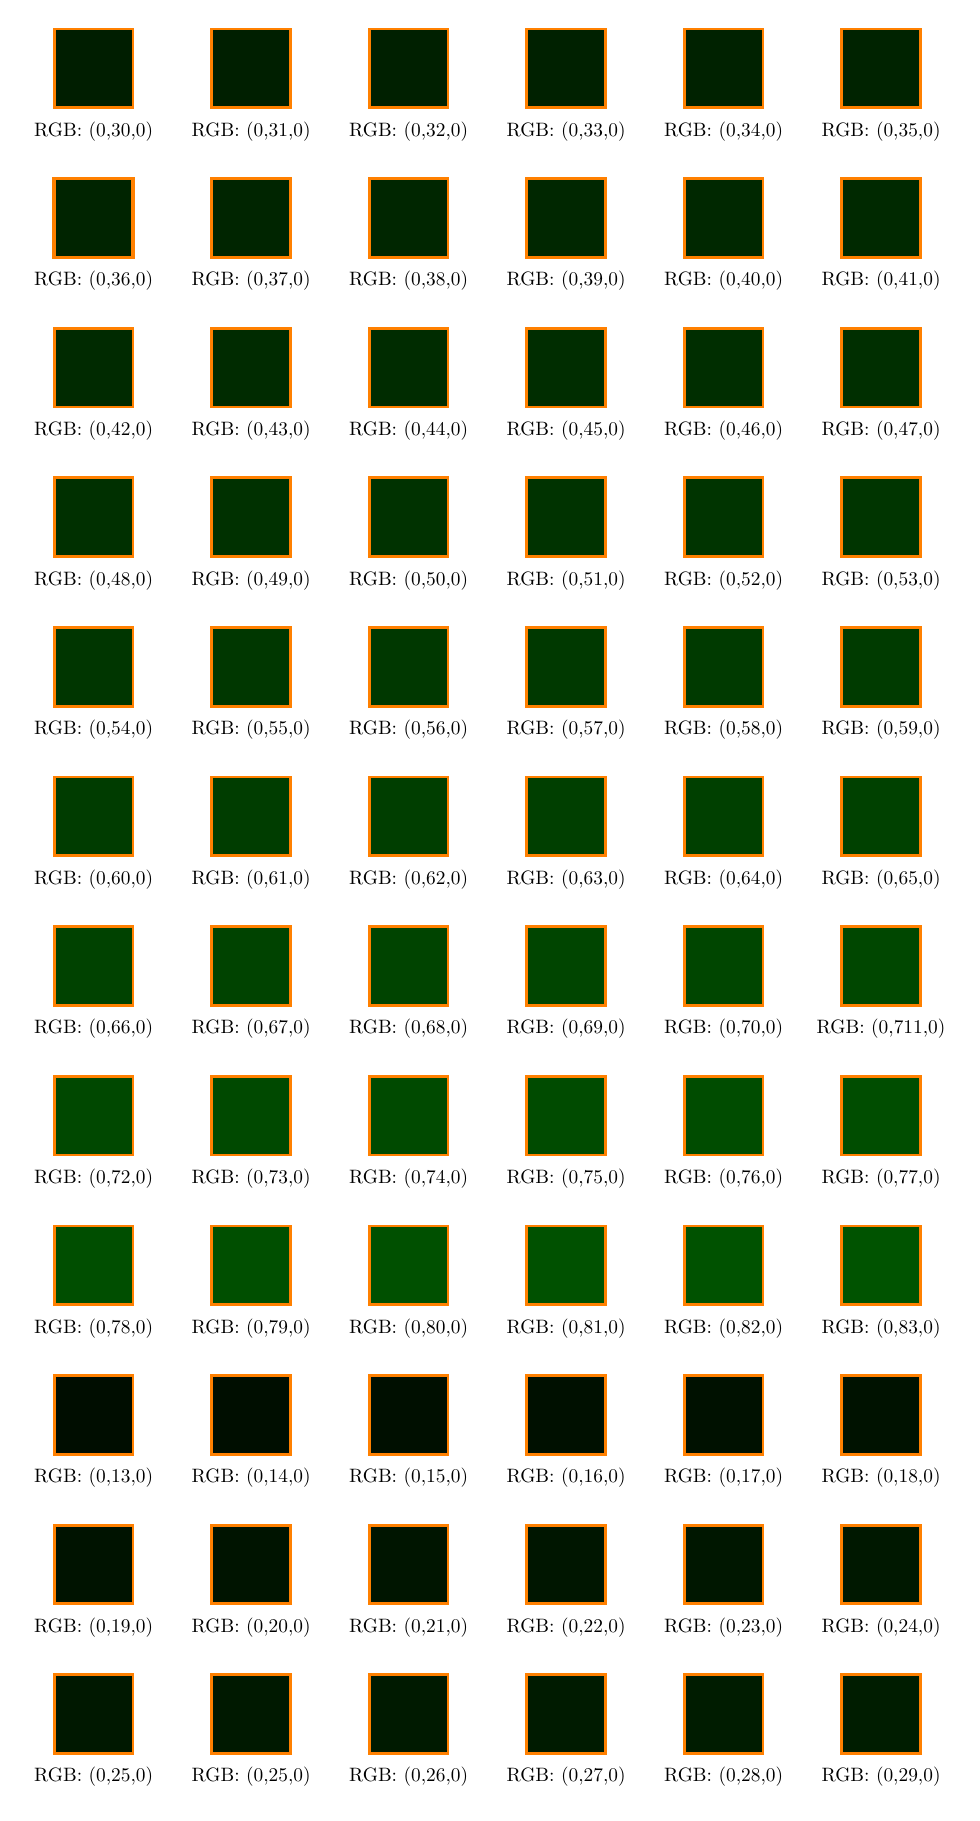
\begin{tikzpicture}

    \filldraw[draw=orange,line width=1,fill=colorR0G30B0]
    (0,0) rectangle (1,1);

    \node[scale=0.7] at (0.5,-0.3) {RGB: (0,30,0)};



    \begin{scope}[xshift=2cm]

      \filldraw[draw=orange,line width=1,fill=colorR0G31B0]
      (0,0) rectangle (1,1);

      \node[scale=0.7] at (0.5,-0.3) {RGB: (0,31,0)};

    \end{scope}



    \begin{scope}[xshift=4cm]

      \filldraw[draw=orange,line width=1,fill=colorR0G32B0]
      (0,0) rectangle (1,1);

      \node[scale=0.7] at (0.5,-0.3) {RGB: (0,32,0)};

    \end{scope}



    \begin{scope}[xshift=6cm]

      \filldraw[draw=orange,line width=1,fill=colorR0G33B0]
      (0,0) rectangle (1,1);

      \node[scale=0.7] at (0.5,-0.3) {RGB: (0,33,0)};

    \end{scope}



    \begin{scope}[xshift=8cm]

      \filldraw[draw=orange,line width=1,fill=colorR0G34B0]
      (0,0) rectangle (1,1);

      \node[scale=0.7] at (0.5,-0.3) {RGB: (0,34,0)};

    \end{scope}



    \begin{scope}[xshift=10cm]

      \filldraw[draw=orange,line width=1,fill=colorR0G35B0]
      (0,0) rectangle (1,1);

      \node[scale=0.7] at (0.5,-0.3) {RGB: (0,35,0)};

    \end{scope}





    \begin{scope}[yshift=-1.9cm]

      \filldraw[draw=orange,line width=1.3,fill=colorR0G36B0]
      (0,0) rectangle (1,1);

      \node[scale=0.7] at (0.5,-0.3) {RGB: (0,36,0)};

    \end{scope}



    \begin{scope}[xshift=2cm,yshift=-1.9cm]

      \filldraw[draw=orange,line width=1,fill=colorR0G37B0]
      (0,0) rectangle (1,1);

      \node[scale=0.7] at (0.5,-0.3) {RGB: (0,37,0)};

    \end{scope}



    \begin{scope}[xshift=4cm,yshift=-1.9cm]

      \filldraw[draw=orange,line width=1,fill=colorR0G38B0]
      (0,0) rectangle (1,1);

      \node[scale=0.7] at (0.5,-0.3) {RGB: (0,38,0)};

    \end{scope}



    \begin{scope}[xshift=6cm,yshift=-1.9cm]

      \filldraw[draw=orange,line width=1,fill=colorR0G39B0]
      (0,0) rectangle (1,1);

      \node[scale=0.7] at (0.5,-0.3) {RGB: (0,39,0)};

    \end{scope}



    \begin{scope}[xshift=8cm,yshift=-1.9cm]

      \filldraw[draw=orange,line width=1,fill=colorR0G40B0]
      (0,0) rectangle (1,1);

      \node[scale=0.7] at (0.5,-0.3) {RGB: (0,40,0)};

    \end{scope}



    \begin{scope}[xshift=10cm,yshift=-1.9cm]

      \filldraw[draw=orange,line width=1,fill=colorR0G41B0]
      (0,0) rectangle (1,1);

      \node[scale=0.7] at (0.5,-0.3) {RGB: (0,41,0)};

    \end{scope}





    \begin{scope}[yshift=-3.8cm]

      \filldraw[draw=orange,line width=1,fill=colorR0G42B0]
      (0,0) rectangle (1,1);

      \node[scale=0.7] at (0.5,-0.3) {RGB: (0,42,0)};

    \end{scope}



    \begin{scope}[xshift=2cm,yshift=-3.8cm]

      \filldraw[draw=orange,line width=1,fill=colorR0G43B0]
      (0,0) rectangle (1,1);

      \node[scale=0.7] at (0.5,-0.3) {RGB: (0,43,0)};

    \end{scope}



    \begin{scope}[xshift=4cm,yshift=-3.8cm]

      \filldraw[draw=orange,line width=1,fill=colorR0G44B0]
      (0,0) rectangle (1,1);

      \node[scale=0.7] at (0.5,-0.3) {RGB: (0,44,0)};

    \end{scope}



    \begin{scope}[xshift=6cm,yshift=-3.8cm]

      \filldraw[draw=orange,line width=1,fill=colorR0G45B0]
      (0,0) rectangle (1,1);

      \node[scale=0.7] at (0.5,-0.3) {RGB: (0,45,0)};

    \end{scope}



    \begin{scope}[xshift=8cm,yshift=-3.8cm]

      \filldraw[draw=orange,line width=1,fill=colorR0G46B0]
      (0,0) rectangle (1,1);

      \node[scale=0.7] at (0.5,-0.3) {RGB: (0,46,0)};

    \end{scope}



    \begin{scope}[xshift=10cm,yshift=-3.8cm]

      \filldraw[draw=orange,line width=1,fill=colorR0G47B0]
      (0,0) rectangle (1,1);

      \node[scale=0.7] at (0.5,-0.3) {RGB: (0,47,0)};

    \end{scope}





    \begin{scope}[yshift=-5.7cm]

      \filldraw[draw=orange,line width=1,fill=colorR0G48B0]
      (0,0) rectangle (1,1);

      \node[scale=0.7] at (0.5,-0.3) {RGB: (0,48,0)};

    \end{scope}



    \begin{scope}[xshift=2cm,yshift=-5.7cm]

      \filldraw[draw=orange,line width=1,fill=colorR0G49B0]
      (0,0) rectangle (1,1);

      \node[scale=0.7] at (0.5,-0.3) {RGB: (0,49,0)};

    \end{scope}



    \begin{scope}[xshift=4cm,yshift=-5.7cm]

      \filldraw[draw=orange,line width=1,fill=colorR0G50B0]
      (0,0) rectangle (1,1);

      \node[scale=0.7] at (0.5,-0.3) {RGB: (0,50,0)};

    \end{scope}



    \begin{scope}[xshift=6cm,yshift=-5.7cm]

      \filldraw[draw=orange,line width=1,fill=colorR0G51B0]
      (0,0) rectangle (1,1);

      \node[scale=0.7] at (0.5,-0.3) {RGB: (0,51,0)};

    \end{scope}



    \begin{scope}[xshift=8cm,yshift=-5.7cm]

      \filldraw[draw=orange,line width=1,fill=colorR0G52B0]
      (0,0) rectangle (1,1);

      \node[scale=0.7] at (0.5,-0.3) {RGB: (0,52,0)};

    \end{scope}



    \begin{scope}[xshift=10cm,yshift=-5.7cm]

      \filldraw[draw=orange,line width=1,fill=colorR0G53B0]
      (0,0) rectangle (1,1);

      \node[scale=0.7] at (0.5,-0.3) {RGB: (0,53,0)};

    \end{scope}





    \begin{scope}[yshift=-7.6cm]

      \filldraw[draw=orange,line width=1,fill=colorR0G54B0]
      (0,0) rectangle (1,1);

      \node[scale=0.7] at (0.5,-0.3) {RGB: (0,54,0)};

    \end{scope}



    \begin{scope}[xshift=2cm,yshift=-7.6cm]

      \filldraw[draw=orange,line width=1,fill=colorR0G55B0]
      (0,0) rectangle (1,1);

      \node[scale=0.7] at (0.5,-0.3) {RGB: (0,55,0)};

    \end{scope}



    \begin{scope}[xshift=4cm,yshift=-7.6cm]

      \filldraw[draw=orange,line width=1,fill=colorR0G56B0]
      (0,0) rectangle (1,1);

      \node[scale=0.7] at (0.5,-0.3) {RGB: (0,56,0)};

    \end{scope}



    \begin{scope}[xshift=6cm,yshift=-7.6cm]

      \filldraw[draw=orange,line width=1,fill=colorR0G57B0]
      (0,0) rectangle (1,1);

      \node[scale=0.7] at (0.5,-0.3) {RGB: (0,57,0)};

    \end{scope}



    \begin{scope}[xshift=8cm,yshift=-7.6cm]

      \filldraw[draw=orange,line width=1,fill=colorR0G58B0]
      (0,0) rectangle (1,1);

      \node[scale=0.7] at (0.5,-0.3) {RGB: (0,58,0)};

    \end{scope}



    \begin{scope}[xshift=10cm,yshift=-7.6cm]

      \filldraw[draw=orange,line width=1,fill=colorR0G59B0]
      (0,0) rectangle (1,1);

      \node[scale=0.7] at (0.5,-0.3) {RGB: (0,59,0)};

    \end{scope}





    \begin{scope}[yshift=-9.5cm]

      \filldraw[draw=orange,line width=1,fill=colorR0G60B0]
      (0,0) rectangle (1,1);

      \node[scale=0.7] at (0.5,-0.3) {RGB: (0,60,0)};

    \end{scope}



    \begin{scope}[xshift=2cm,yshift=-9.5cm]

      \filldraw[draw=orange,line width=1,fill=colorR0G61B0]
      (0,0) rectangle (1,1);

      \node[scale=0.7] at (0.5,-0.3) {RGB: (0,61,0)};

    \end{scope}



    \begin{scope}[xshift=4cm,yshift=-9.5cm]

      \filldraw[draw=orange,line width=1,fill=colorR0G62B0]
      (0,0) rectangle (1,1);

      \node[scale=0.7] at (0.5,-0.3) {RGB: (0,62,0)};

    \end{scope}



    \begin{scope}[xshift=6cm,yshift=-9.5cm]

      \filldraw[draw=orange,line width=1,fill=colorR0G63B0]
      (0,0) rectangle (1,1);

      \node[scale=0.7] at (0.5,-0.3) {RGB: (0,63,0)};

    \end{scope}



    \begin{scope}[xshift=8cm,yshift=-9.5cm]

      \filldraw[draw=orange,line width=1,fill=colorR0G64B0]
      (0,0) rectangle (1,1);

      \node[scale=0.7] at (0.5,-0.3) {RGB: (0,64,0)};

    \end{scope}



    \begin{scope}[xshift=10cm,yshift=-9.5cm]

      \filldraw[draw=orange,line width=1,fill=colorR0G65B0]
      (0,0) rectangle (1,1);

      \node[scale=0.7] at (0.5,-0.3) {RGB: (0,65,0)};

    \end{scope}





    \begin{scope}[yshift=-11.4cm]

      \filldraw[draw=orange,line width=1,fill=colorR0G66B0]
      (0,0) rectangle (1,1);

      \node[scale=0.7] at (0.5,-0.3) {RGB: (0,66,0)};

    \end{scope}



    \begin{scope}[xshift=2cm,yshift=-11.4cm]

      \filldraw[draw=orange,line width=1,fill=colorR0G67B0]
      (0,0) rectangle (1,1);

      \node[scale=0.7] at (0.5,-0.3) {RGB: (0,67,0)};

    \end{scope}



    \begin{scope}[xshift=4cm,yshift=-11.4cm]

      \filldraw[draw=orange,line width=1,fill=colorR0G68B0]
      (0,0) rectangle (1,1);

      \node[scale=0.7] at (0.5,-0.3) {RGB: (0,68,0)};

    \end{scope}



    \begin{scope}[xshift=6cm,yshift=-11.4cm]

      \filldraw[draw=orange,line width=1,fill=colorR0G69B0]
      (0,0) rectangle (1,1);

      \node[scale=0.7] at (0.5,-0.3) {RGB: (0,69,0)};

    \end{scope}



    \begin{scope}[xshift=8cm,yshift=-11.4cm]

      \filldraw[draw=orange,line width=1,fill=colorR0G70B0]
      (0,0) rectangle (1,1);

      \node[scale=0.7] at (0.5,-0.3) {RGB: (0,70,0)};

    \end{scope}



    \begin{scope}[xshift=10cm,yshift=-11.4cm]

      \filldraw[draw=orange,line width=1,fill=colorR0G71B0]
      (0,0) rectangle (1,1);

      \node[scale=0.7] at (0.5,-0.3) {RGB: (0,711,0)};

    \end{scope}





    \begin{scope}[yshift=-13.3cm]

      \filldraw[draw=orange,line width=1,fill=colorR0G72B0]
      (0,0) rectangle (1,1);

      \node[scale=0.7] at (0.5,-0.3) {RGB: (0,72,0)};

    \end{scope}



    \begin{scope}[xshift=2cm,yshift=-13.3cm]

      \filldraw[draw=orange,line width=1,fill=colorR0G73B0]
      (0,0) rectangle (1,1);

      \node[scale=0.7] at (0.5,-0.3) {RGB: (0,73,0)};

    \end{scope}



    \begin{scope}[xshift=4cm,yshift=-13.3cm]

      \filldraw[draw=orange,line width=1,fill=colorR0G74B0]
      (0,0) rectangle (1,1);

      \node[scale=0.7] at (0.5,-0.3) {RGB: (0,74,0)};

    \end{scope}



    \begin{scope}[xshift=6cm,yshift=-13.3cm]

      \filldraw[draw=orange,line width=1,fill=colorR0G75B0]
      (0,0) rectangle (1,1);

      \node[scale=0.7] at (0.5,-0.3) {RGB: (0,75,0)};

    \end{scope}



    \begin{scope}[xshift=8cm,yshift=-13.3cm]

      \filldraw[draw=orange,line width=1,fill=colorR0G76B0]
      (0,0) rectangle (1,1);

      \node[scale=0.7] at (0.5,-0.3) {RGB: (0,76,0)};

    \end{scope}



    \begin{scope}[xshift=10cm,yshift=-13.3cm]

      \filldraw[draw=orange,line width=1,fill=colorR0G77B0]
      (0,0) rectangle (1,1);

      \node[scale=0.7] at (0.5,-0.3) {RGB: (0,77,0)};

    \end{scope}





    \begin{scope}[yshift=-15.2cm]

      \filldraw[draw=orange,line width=1,fill=colorR0G78B0]
      (0,0) rectangle (1,1);

      \node[scale=0.7] at (0.5,-0.3) {RGB: (0,78,0)};

    \end{scope}



    \begin{scope}[xshift=2cm,yshift=-15.2cm]

      \filldraw[draw=orange,line width=1,fill=colorR0G79B0]
      (0,0) rectangle (1,1);

      \node[scale=0.7] at (0.5,-0.3) {RGB: (0,79,0)};

    \end{scope}



    \begin{scope}[xshift=4cm,yshift=-15.2cm]

      \filldraw[draw=orange,line width=1,fill=colorR0G80B0]
      (0,0) rectangle (1,1);

      \node[scale=0.7] at (0.5,-0.3) {RGB: (0,80,0)};

    \end{scope}



    \begin{scope}[xshift=6cm,yshift=-15.2cm]

      \filldraw[draw=orange,line width=1,fill=colorR0G81B0]
      (0,0) rectangle (1,1);

      \node[scale=0.7] at (0.5,-0.3) {RGB: (0,81,0)};

    \end{scope}



    \begin{scope}[xshift=8cm,yshift=-15.2cm]

      \filldraw[draw=orange,line width=1,fill=colorR0G82B0]
      (0,0) rectangle (1,1);

      \node[scale=0.7] at (0.5,-0.3) {RGB: (0,82,0)};

    \end{scope}



    \begin{scope}[xshift=10cm,yshift=-15.2cm]

      \filldraw[draw=orange,line width=1,fill=colorR0G83B0]
      (0,0) rectangle (1,1);

      \node[scale=0.7] at (0.5,-0.3) {RGB: (0,83,0)};

    \end{scope}





    \begin{scope}[yshift=-17.1cm]

      \filldraw[draw=orange,line width=1,fill=colorR0G13B0]
      (0,0) rectangle (1,1);

      \node[scale=0.7] at (0.5,-0.3) {RGB: (0,13,0)};

    \end{scope}



    \begin{scope}[xshift=2cm,yshift=-17.1cm]

      \filldraw[draw=orange,line width=1,fill=colorR0G14B0]
      (0,0) rectangle (1,1);

      \node[scale=0.7] at (0.5,-0.3) {RGB: (0,14,0)};

    \end{scope}



    \begin{scope}[xshift=4cm,yshift=-17.1cm]

      \filldraw[draw=orange,line width=1,fill=colorR0G15B0]
      (0,0) rectangle (1,1);

      \node[scale=0.7] at (0.5,-0.3) {RGB: (0,15,0)};

    \end{scope}



    \begin{scope}[xshift=6cm,yshift=-17.1cm]

      \filldraw[draw=orange,line width=1,fill=colorR0G16B0]
      (0,0) rectangle (1,1);

      \node[scale=0.7] at (0.5,-0.3) {RGB: (0,16,0)};

    \end{scope}



    \begin{scope}[xshift=8cm,yshift=-17.1cm]

      \filldraw[draw=orange,line width=1,fill=colorR0G17B0]
      (0,0) rectangle (1,1);

      \node[scale=0.7] at (0.5,-0.3) {RGB: (0,17,0)};

    \end{scope}



    \begin{scope}[xshift=10cm,yshift=-17.1cm]

      \filldraw[draw=orange,line width=1,fill=colorR0G18B0]
      (0,0) rectangle (1,1);

      \node[scale=0.7] at (0.5,-0.3) {RGB: (0,18,0)};

    \end{scope}





    \begin{scope}[yshift=-19cm]

      \filldraw[draw=orange,line width=1,fill=colorR0G19B0]
      (0,0) rectangle (1,1);

      \node[scale=0.7] at (0.5,-0.3) {RGB: (0,19,0)};

    \end{scope}



    \begin{scope}[xshift=2cm,yshift=-19cm]

      \filldraw[draw=orange,line width=1,fill=colorR0G20B0]
      (0,0) rectangle (1,1);

      \node[scale=0.7] at (0.5,-0.3) {RGB: (0,20,0)};

    \end{scope}



    \begin{scope}[xshift=4cm,yshift=-19cm]

      \filldraw[draw=orange,line width=1,fill=colorR0G21B0]
      (0,0) rectangle (1,1);

      \node[scale=0.7] at (0.5,-0.3) {RGB: (0,21,0)};

    \end{scope}



    \begin{scope}[xshift=6cm,yshift=-19cm]

      \filldraw[draw=orange,line width=1,fill=colorR0G22B0]
      (0,0) rectangle (1,1);

      \node[scale=0.7] at (0.5,-0.3) {RGB: (0,22,0)};

    \end{scope}



    \begin{scope}[xshift=8cm,yshift=-19cm]

      \filldraw[draw=orange,line width=1,fill=colorR0G23B0]
      (0,0) rectangle (1,1);

      \node[scale=0.7] at (0.5,-0.3) {RGB: (0,23,0)};

    \end{scope}



    \begin{scope}[xshift=10cm,yshift=-19cm]

      \filldraw[draw=orange,line width=1,fill=colorR0G24B0]
      (0,0) rectangle (1,1);

      \node[scale=0.7] at (0.5,-0.3) {RGB: (0,24,0)};

    \end{scope}





    \begin{scope}[yshift=-20.9cm]

      \filldraw[draw=orange,line width=1,fill=colorR0G24B0]
      (0,0) rectangle (1,1);

      \node[scale=0.7] at (0.5,-0.3) {RGB: (0,25,0)};

    \end{scope}



    \begin{scope}[xshift=2cm,yshift=-20.9cm]

      \filldraw[draw=orange,line width=1,fill=colorR0G25B0]
      (0,0) rectangle (1,1);

      \node[scale=0.7] at (0.5,-0.3) {RGB: (0,25,0)};

    \end{scope}



    \begin{scope}[xshift=4cm,yshift=-20.9cm]

      \filldraw[draw=orange,line width=1,fill=colorR0G26B0]
      (0,0) rectangle (1,1);

      \node[scale=0.7] at (0.5,-0.3) {RGB: (0,26,0)};

    \end{scope}



    \begin{scope}[xshift=6cm,yshift=-20.9cm]

      \filldraw[draw=orange,line width=1,fill=colorR0G27B0]
      (0,0) rectangle (1,1);

      \node[scale=0.7] at (0.5,-0.3) {RGB: (0,27,0)};

    \end{scope}



    \begin{scope}[xshift=8cm,yshift=-20.9cm]

      \filldraw[draw=orange,line width=1,fill=colorR0G28B0]
      (0,0) rectangle (1,1);

      \node[scale=0.7] at (0.5,-0.3) {RGB: (0,28,0)};

    \end{scope}



    \begin{scope}[xshift=10cm,yshift=-20.9cm]

      \filldraw[draw=orange,line width=1,fill=colorR0G29B0]
      (0,0) rectangle (1,1);

      \node[scale=0.7] at (0.5,-0.3) {RGB: (0,29,0)};

    \end{scope}

  \end{tikzpicture}

  \caption{Główne składowe kolorów w~systemie~RGB: $(0,30,0)$--$(0,???,0)$}



  \label{fig:Basic-colors-Part-05}

\end{figure}
% ##################











% ####################################################################
% ####################################################################
% Bibliography

% \printbibliography





% ############################
% End of the document

\end{document}
